%%%% Шаблон ВКР <<SPbPU-student-thesis-template>>  %%%%
%%
%%   Создан на основе глубокой переработки шаблона российских кандидатских и докторских диссертаций [1]. 
%%   
%%   Полный список различий может быть получен командами git.
%%   Лист авторов-составителей расположен в README.md файле.
%%   Подробные инструкции по использованию в [1,2].
%%   
%%   Рекомендуем установить TeX Live + TeXstudio
%%   <<Стандартная>> компиляция 2-3 РАЗА с помощью pdflatex + biber (для библиографии)     
%%  
%%%% Student thesis template <<SPbPU-student-thesis-template>> %%%%
%%
%%   Created on the basis of deepl modifification of the Russian candidate and doctorate thesis template [1]. 
%%   
%%   Full list of differences can be achieved by git commands.
%%   List of template authors can be seen in the README.md file.
%%   Detailed instructions of usage, see, please in [1,2].
%%     
%%   [1] github.com/AndreyAkinshin/Russian-Phd-LaTeX-Dissertation-Template 
%%   [2] Author_guide_SPBPU-student-thesis-template.pdf
%%   
%%   It is recommended to install TeX Live + TeXstudio   
%%   Default compilation 2-3 TIMES with pdflatex + biber (for the bibliography)
%%  
\input{template_settings/ch_preamble} % лучше не редактировать / please, keep unmodified

\setcounter{docType}{1} % лучше не редактировать / please, keep unmodified

%%%% Настройки автора / Author settings
%% 
\input{my_folder/my_settings} % добавляем свои команды / update your commands

\begin{document} % начало документа


%%% Внесите свои данные - Input your data
%%
%%
\newcommand{\Author}{К.А. Дамасинский} % И.О. Фамилия автора 
\newcommand{\AuthorFull}{Дамаскинский Константин Александрович} % Фамилия Имя Отчество автора
\newcommand{\AuthorFullDat}{Дамаскинскому Константину Александровичу} % Фамилия Имя Отчество автора в дательном падеже (Кому? Студенту...)
\newcommand{\AuthorFullVin}{Дамаскинского Константина Александровича} % в винительном падеже (Кого? что?  Програмиста ...)
\newcommand{\AuthorPhone}{+7-911-135-40-48} % номер телефорна автора для оперативной связи  
\newcommand{\Supervisor}{В.С. Чуканов} % И. О. Фамилия научного руководителя
\newcommand{\SupervisorFull}{Вячеслав Сергеевич Чуканов} % Фамилия Имя Отчество научного руководителя
\newcommand{\SupervisorVin}{В.С. Чуканова} % И. О. Фамилия научного руководителя  в винительном падеже (Кого? что? Руководителя ...)
\newcommand{\SupervisorJob}{старший преподаватель ВШПМиВФ} %
\newcommand{\SupervisorJobVin}{старшего преподавателя ВШПМиВФ} % в винительном падеже (Кого? что?  Програмиста ...)
\newcommand{\SupervisorDegree}{} %
\newcommand{\SupervisorTitle}{} % 
%%
%%
%Руководитель, утверждающий задание
\newcommand{\Head}{К.Н. Козлов} % И. О. Фамилия руководителя подразделения (руководителя ОП)
\newcommand{\HeadDegree}{Руководитель ОП}% Только должность:   
%Руководитель %ОП 
%Заведующий % кафедрой
%Директор % Высшей школы
%Зам. директора
\newcommand{\HeadDep}{} % заменить на краткую аббревиатуру подразделения или оставить пустым, если утверждает руководитель ОП

%%% Руководитель, принимающий заявление
\newcommand{\HeadAp}{К.Н. Козлов} % И. О. Фамилия руководителя подразделения (руководителя ОП)
\newcommand{\HeadApDegree}{Руководитель ОП}% Только должность:   
%Руководитель ОП 
%Заведующий кафедрой
%Директор Высшей школы
\newcommand{\HeadApDep}{} % заменить на краткую аббревиатуру подразделения или оставить пустым, если утверждает руководитель ОП
%%% Консультант по нормоконтролю
\newcommand{\ConsultantNorm}{Л.А. Арефьева} % И. О. Фамилия консультанта по нормоконтролю. ТОЛЬКО из числа ППС!
\newcommand{\ConsultantNormDegree}{} %   
%%% Первый консультант
%\newcommand{\ConsultantExtraFull}{Фамилия Имя Отчетство} % Фамилия Имя Отчетство дополнительного консультанта 
%\newcommand{\ConsultantExtra}{И.О.\,Фамилия} % И. О. Фамилия дополнительного консультанта 
%\newcommand{\ConsultantExtraDegree}{должность, степень} % 
%\newcommand{\ConsultantExtraVin}{И.О.\,Фамилию} % И. О. Фамилия дополнительного консультанта в винительном падеже (Кого? что? Руководителя ...)
%\newcommand{\ConsultantExtraDegreeVin}{должность, степень} %  в винительном падеже (Кого? что? Руководителя ...)
%%% Второй консультант
%\newcommand{\ConsultantExtraTwoFull}{Фамилия Имя Отчетство} % Фамилия Имя Отчетство дополнительного консультанта 
%\newcommand{\ConsultantExtraTwo}{И.О.\,Фамилия} % И. О. Фамилия дополнительного консультанта 
%\newcommand{\ConsultantExtraTwoDegree}{должность, степень} % 
%\newcommand{\ConsultantExtraTwoVin}{И.О.\,Фамилию} % И. О. Фамилия дополнительного консультанта в винительном падеже (Кого? что? Руководителя ...)
%\newcommand{\ConsultantExtraTwoDegreeVin}{должность, степень} %  в винительном падеже (Кого? что? Руководителя ...)
%\newcommand{\Reviewer}{И.О.\,Фамилия} % И. О. Фамилия резензента. Обязателен только для магистров.
%\newcommand{\ReviewerDegree}{должность, степень} % 
%%
%%
\renewcommand{\thesisTitle}{Распознавание химической структуры молекулы методами машинного обучения}
\newcommand{\thesisDegree}{магистерская диссертация}% дипломный проект, дипломная работа, магистерская диссертация %c 2020
\newcommand{\thesisTitleEn}{Molecular structure detection by machine learning methods} %2020
\newcommand{\thesisDeadline}{июнь 2023}
\newcommand{\thesisStartDate}{13.02.2023}
\newcommand{\thesisYear}{2023}
%%
%%
\newcommand{\group}{5040102/10201} % заменить вместо N номер группы
\newcommand{\thesisSpecialtyCode}{01.04.02}% код направления подготовки
\newcommand{\thesisSpecialtyTitle}{Прикладная математика и информатика} % наименование направления/специальности
\newcommand{\thesisOPPostfix}{02} % последние цифры кода образовательной программы (после <<_>>)
\newcommand{\thesisOPTitle}{Математические методы анализа и визуализации данных}% наименование образовательной программы
%%
%%
\newcommand{\institute}{
Физико-механический институт
%Институт компьютерных наук и~технологий
%Гуманитарный институт
%Инженерно-строительный институт
%Институт биомедицинских систем и технологий
%Институт металлургии, машиностроения и транспорта
%Институт передовых производственных технологий
%Институт прикладной математики и механики
%Институт физики, нанотехнологий и телекоммуникаций
%Институт физической культуры, спорта и туризма
%Институт энергетики и транспортных систем
%Институт промышленного менеджмента, экономики и торговли
}%
%%
%%




%%% Задание ключевых слов и аннотации
%%
%%
%% Ключевых слов от 3 до 5 слов или словосочетаний в именительном падеже именительном падеже множественного числа (или в единственном числе, если нет другой формы) по правилам русского языка!!!
%%
%%
\newcommand{\keywordsRu}{Задача распознавания, химия, InChI, машинное обучение} % ВВЕДИТЕ ключевые слова по-русски
%%
%%
\newcommand{\keywordsEn}{Object detection, chemistry, InChI, machine learning} % ВВЕДИТЕ ключевые слова по-английски
%%
%%
%% Реферат ОТ 1000 ДО 1500 знаков на русский или английский текст
%%
%Реферат должен содержать:
%- предмет, тему, цель ВКР;
%- метод или методологию проведения ВКР:
%- результаты ВКР:
%- область применения результатов ВКР;
%- выводы.

\newcommand{\abstractRu}{В данной работе изложена сущность подхода к созданию динамического информационного портала на основе использования открытых технологий Apache, MySQL и PHP. Даны общие понятия и классификация IT-систем такого класса. Проведен анализ систем-прототипов. Изучена технология создания указанного класса информационных систем. Разработана конкретная программная реализация динамического информационного портала на примере портала выбранной тематики...} % ВВЕДИТЕ текст аннотации по-русски
%%
%%
\newcommand{\abstractEn}{In the given work the essence of the approach to creation of a dynamic information portal on the basis of use of open technologies Apache, MySQL and PHP is stated. The general concepts and classification of IT-systems of such class are given. The analysis of systems-prototypes is lead. The technology of creation of the specified class of information systems is investigated. Concrete program realization of a dynamic information portal on an example of a portal of the chosen subjects is developed...} % ВВЕДИТЕ текст аннотации по-английски


%%% РАЗДЕЛ ДЛЯ ОФОРМЛЕНИЯ ПРАКТИКИ
%Место прохождения практики
\newcommand{\PracticeType}{Отчет о прохождении производственной практики}

\newcommand{\Workplace}{СПбПУ, ФМИ, ВШПМиВФ} % TODO Rename this variable

% Даты начала/окончания
\newcommand{\PracticeStartDate}{%
01.02.2023%
%	22.06.2020
}%
\newcommand{\PracticeEndDate}{%
	01.05.2023
}%
%%

\newcommand{\School}{
	Высшая школа прикладной математики и вычислительной физики
}
\newcommand{\practiceTitle}{Распознавание структуры химической молекулы методами машинного обучения}


%% ВНИМАНИЕ! Необходимо либо заменить текст аннотации (ключевых слов) на русском и английском, либо удалить там весь текст, иначе в свойства pdf-отчета по практике пойдет шаблонный текст.

%%% Не меняем дальнейшую часть - Do not modify the rest part
%%
%%
%%
%%
\ifnumequal{\value{docType}}{1}{% Если ВКР, то...
	\newcommand{\DocType}{Выпускная квалификационная работа}
	\newcommand{\pdfDocType}{\DocType~(\thesisDegree)} %задаём метаданные pdf файла
	\newcommand{\pdfTitle}{\thesisTitle}
}{% Иначе 
	\newcommand{\DocType}{\PracticeType}
	\newcommand{\pdfDocType}{\DocType} %задаём метаданные pdf файла
	\newcommand{\pdfTitle}{\practiceTitle}
}%
\newcommand{\HeadTitle}{\HeadDegree~\HeadDep}
\newcommand{\HeadApTitle}{\HeadApDegree~\HeadApDep}
\newcommand{\thesisOPCode}{\thesisSpecialtyCode\_\thesisOPPostfix}% код образовательной программы
\newcommand{\thesisSpecialtyCodeAndTitle}{\thesisSpecialtyCode~\thesisSpecialtyTitle}% Код и наименование направления/специальности
\newcommand{\thesisOPCodeAndTitle}{\thesisOPCode~\thesisOPTitle} % код и наименование образовательной программы
%%
%%
\hypersetup{%часть болка hypesetup в style
		pdftitle={\pdfTitle},    % Заголовок pdf-файла
		pdfauthor={\AuthorFull},    % Автор
		pdfsubject={\pdfDocType. Шифр и наименование направления подготовки: \thesisSpecialtyCodeAndTitle. \abstractRu},      % Тема
		pdfcreator={LaTeX, SPbPU-student-thesis-template},     % Приложение-создатель
%		pdfproducer={},  % Производитель, Производитель PDF % будет выставлена автоматически
		pdfkeywords={\keywordsRu}
}
%%
%%
%% вспомогательные команды
\newcommand{\firef}[1]{рис.\ref{#1}} %figure reference
\newcommand{\taref}[1]{табл.\ref{#1}}	%table reference
%%
%%
%% Архивный вариант задания ключевых слов, аннотации и благодарностей 
% Too hard to export data from the environment to pdf-info
% https://tex.stackexchange.com/questions/184503/collecting-contents-of-environment-and-store-them-for-later-retrieval
%заменить NewEnviron на newenvironment для распознавания команды в TexStudio
%\NewEnviron{keywordsRu}{\noindent\MakeUppercase{\BODY}}
%\NewEnviron{keywordsEn}{\noindent\MakeUppercase{\BODY}}
%\newenvironment{abstractRu}{}{}
%\newenvironment{abstractEn}{}{}
%\newenvironment{acknowledgementsRu}{\par{\normalfont \acknowledgements.}}{}
%\newenvironment{acknowledgementsEn}{\par{\normalfont \acknowledgementsENG.}}{}


%%% Переопределение именований %%% Не меняем - Do not modify
%\newcommand{\Ministry}{Минобрнауки России} 
\newcommand{\Ministry}{Министерство науки и высшего образования Российской~Федерации} %с 2020
\newcommand{\SPbPU}{Санкт-Петербургский политехнический университет Петра~Великого}
\newcommand{\SPbPUOfficialPrefix}{Федеральное государственное автономное образовательное учреждение высшего образования}
\newcommand{\SPbPUOfficialShort}{ФГАОУ~ВО~<<СПбПУ>>}
%% Пробел между И. О. не допускается.
\renewcommand{\alsoname}{см. также}
\renewcommand{\seename}{см.}
\renewcommand{\headtoname}{вх.}
\renewcommand{\ccname}{исх.}
\renewcommand{\enclname}{вкл.}
\renewcommand{\pagename}{Pages}
\renewcommand{\partname}{Часть}
\renewcommand{\abstractname}{\textbf{Аннотация}}
\newcommand{\abstractnameENG}{\textbf{Annotation}}
\newcommand{\keywords}{\textbf{Ключевые слова}}
\newcommand{\keywordsENG}{\textbf{Keywords}}
\newcommand{\acknowledgements}{\textbf{Благодарности}}
\newcommand{\acknowledgementsENG}{\textbf{Acknowledgements}}
\renewcommand{\contentsname}{Content} % 
%\renewcommand{\contentsname}{Содержание} % (ГОСТ Р 7.0.11-2011, 4)
%\renewcommand{\contentsname}{Оглавление} % (ГОСТ Р 7.0.11-2011, 4)
\renewcommand{\figurename}{Рис.} % Стиль СПбПУ
%\renewcommand{\figurename}{Рисунок} % (ГОСТ Р 7.0.11-2011, 5.3.9)
\renewcommand{\tablename}{Таблица} % (ГОСТ Р 7.0.11-2011, 5.3.10)
%\renewcommand{\indexname}{Предметный указатель}
\renewcommand{\listfigurename}{Список рисунков}
\renewcommand{\listtablename}{Список таблиц}
\renewcommand{\refname}{\fullbibtitle}
\renewcommand{\bibname}{\fullbibtitle}

\newcommand{\chapterEnTitle}{Сhapter title} % <- input the English title here (only once!) 
\newcommand{\chapterRuTitle}{Название главы}          % <- введите 
\newcommand{\sectionEnTitle}{Section title} %<- input subparagraph title in english
\newcommand{\sectionRuTitle}{Название подраздела} % <- введите название подраздела по-русски
\newcommand{\subsectionEnTitle}{Subsection title} % - input subsection title in english
\newcommand{\subsectionRuTitle}{Название параграфа} % <- введите название параграфа по-русски
\newcommand{\subsubsectionEnTitle}{Subsubsection title} % <- input subparagraph title in english
\newcommand{\subsubsectionRuTitle}{Название подпараграфа} % <- введите название подпараграфа по-русски % Заполнить сведения, 
										 % в т.ч. ключевые слова и аннотацию.

%%% Титульник ВКР / Thesis title 
%%
%% добавить лист в pdf-навигацию 
%% add to pdf navigation menu
%%
\pdfbookmark[-1]{\pdfTitle}{tit}
%%
\thispagestyle{empty}%
\makeatletter
\newgeometry{top=2cm,bottom=2cm,left=3cm,right=1cm,headsep=0cm,footskip=0cm}
\savegeometry{NoFoot}%
\makeatother


%%% Распечатать версию документа / Print document version
%%
%\begin{flushright}
%%	\vspace{0pt plus0.1fill}
%	\boxed{\small
%		\begin{tabular}{r} 
%			\textbf{Пример ВКР <<SPbPU-student-thesis-template>>.} %\\ % перенос на новую строку
%			\textbf{Версия от \today % \; время:  \currenttime. % время версии
%			}
%		\end{tabular}
%	} %end boxed
%%	\vspace*{-5pt} % раскомментировать, если не хватает места
%	\vspace{0pt plus0.1fill} % раскоментировать, если хватает места
%\end{flushright}

{\centering%
	\Ministry\\
	\SPbPU\\
	{%\bfseries %2020 - указание на изменения, которые могут быть введены в 2020 году
		\institute}
\par}%


\vspace{0pt plus1fill} %число перед fill = кратность относительно некоторого расстояния fill, кусками которого заполнены пустые места


\noindent
\begin{minipage}{\linewidth}
	\vspace{\mfloatsep} % интервал 
	\begin{tabularx}{\linewidth}{Xl}
	&Работа допущена к защите     \\
	&\HeadTitle     \\			
	&\underline{\hspace*{0.1\textheight}} \Head     \\
	&<<\underline{\hspace*{0.05\textheight}}>> \underline{\hspace*{0.1\textheight}} \thesisYear~г.  \\ 
	\end{tabularx}
	\vspace{\mfloatsep} % интервал 	
\end{minipage}


\vspace{0pt plus2fill} %


{\centering%
	
	\MakeUppercase{\bfseries{}\DocType} \\ 
	\MakeUppercase{\thesisDegree}%


%\intervalS% %ОБЯЗАТЕЛЬНО ДОБАВИТЬ ОТСТУП, ЕСЛИ ХВАТАЕТ МЕСТА
{\centering%
	\MakeUppercase{\bfseries{\thesisTitle}}}%

}\par%

%\intervalS% %ОБЯЗАТЕЛЬНО ДОБАВИТЬ ОТСТУП, ЕСЛИ ХВАТАЕТ МЕСТА
%по специальности % для специалистов
\noindent	по направлению подготовки \thesisSpecialtyCodeAndTitle{}\\% для бакалавров и магистров 
%\noindent Направленность  % для специалистов
\noindent	Направленность (профиль)	\thesisOPCodeAndTitle % для бакалавров и магистров
% Лучше по~профилю, но что делать, так составили Положение
\par%





\vspace{4mm plus2fill}%

\noindent
\begin{tabularx}{\linewidth}{lXl}
	Выполнил              &	   &             \\
	студент гр.~\group     &    & \Author     \\[\mfloatsep]

	Руководитель 		  &    &             \\
	\SupervisorJob		  &    &             \\
	\SupervisorDegree \SupervisorTitle 	  &    & \Supervisor \\[\mfloatsep]
	
	
	Консультант  &    &  \\   	
	по нормоконтролю  		 	  &    & \ConsultantNorm  % обязателен
\end{tabularx} %


%
\vspace{0pt plus4fill}% 


\begin{center}%
Санкт-Петербург\\
\thesisYear
\end{center}%
\restoregeometry
\newpage					 % Титульный лист
										 % Убираем footnotes, консультанта, если нет

%%%% Начало оформления заголовка - оставить без изменений !!! %%%%
\input{my_folder/task_settings}	% настройки - начало 
	
				{%\normalfont %2020
						\MakeUppercase{\SPbPU}}\\
				\institute

\par}\intervalS% завершает input

				\noindent
				\begin{minipage}{\linewidth}
				\vspace{\mfloatsep} % интервал 	
				\begin{tabularx}{\linewidth}{Xl}
					&УТВЕРЖДАЮ      \\
					&\HeadTitle     \\			
					&\underline{\hspace*{0.1\textheight}} \Head     \\
					&<<\underline{\hspace*{0.05\textheight}}>> \underline{\hspace*{0.1\textheight}} \thesisYear г.  \\  
				\end{tabularx}
				\vspace{\mfloatsep} % интервал 	
				\end{minipage}

\intervalS{\centering\bfseries%

				ЗАДАНИЕ\\
				на выполнение %с 2020 года 
				%по выполнению % до 2020 года
				выпускной квалификационной работы


\intervalS\normalfont%

				студенту \uline{\AuthorFullDat{} гр.~\group}


\par}\intervalS%
%%%%
%%%% Конец оформления заголовка  %%%%
 	
	
	
\begin{enumerate}[1.]
	\item Тема работы: {\expandafter \ulined \thesisTitle.}
	%\item Тема работы (на английском языке): \uline{\thesisTitleEn.} % вероятно после 2021 года
	\item Срок сдачи студентом законченной работы\: \uline{\thesisDeadline.} 
	\item Исходные данные по работе\: 
	\begin{itemize}
		\item Набор молекул, сохранённых в InChI формате, полученный из kaggle соревнования BMS \cite{bms}.
		\item Обзорные статьи:
		\begin{enumerate}
			\item OCR-решения для распознавания молекул: \cite{vogt2022using}
			\item ML-решения для распознавания молекул: \cite{vogt2022using}
		\end{enumerate}
		\item Инструментальные средства:
		\begin{itemize}
			\item Языки программирования С++, Python, bash
			\item Платформа для машинного обучения Google Cloud
			\item Система контроля версий git
		\end{itemize}
	\end{itemize}
	\printbibliographyTask % печать списка источников % КОММЕНТИРУЕМ ЕСЛИ НЕ ИСПОЛЬЗУЕТСЯ
	% В СЛУЧАЕ, ЕСЛИ НЕ ИСПОЛЬЗУЕТСЯ МОЖНО ТАКЖЕ ЗАЙТИ В setup.tex и закомментировать \vspace{-0.28\curtextsize}
	\item Содержание работы (перечень подлежащих разработке вопросов):
	\begin{enumerate}[label=\theenumi\arabic*.]
		\item Введение. Обоснование актуальности
		\item Постановка задачи
		\item Обзор существующих решений
		\item Разработка моделей машинного обучения
		\item Применение
		\item Результаты и их сравнительный анализ
		\item Выводы
		\item Заключение
	\end{enumerate}
		%\item Консультанты по работе\footnote{Подпись консультанта по нормоконтролю пока не требуется. Назначается всем по умолчанию.}:
		%\begin{enumerate}[label=\theenumi\arabic*.] 
		%\item  \uline{\emakefirstuc{\ConsultantExtraDegree}, \ConsultantExtra.} % закомментировать при необходимости, идёт первый по порядку.
		%\item \uline{\emakefirstuc{\ConsultantNormDegree}, \ConsultantNorm{} (нормоконтроль).} %	Обязателен для всех студентов
	%\end{enumerate}
		\item Дата выдачи задания: \uline{\thesisStartDate.}
\end{enumerate}

\intervalS%можно удалить пробел

Руководитель ВКР \uline{\hspace*{0.1\textheight} \Supervisor}


\intervalS%можно удалить пробел

%Консультант\footnote{В случае, если есть консультант, отличный от консультанта по нормоконтролю.}  \uline{\hspace*{0.1\textheight}\ConsultantExtra}


\intervalS%можно удалить пробел

%Консультант по нормоконтролю \uline{\hspace*{0.1\textheight} \ConsultantNorm}%ПОКА НЕ ТРЕБУЕТСЯ, Т.К. ОН У ВСЕХ ПО УМОЛЧАНИЮ

Задание принял к исполнению \uline{\thesisStartDate}

\intervalS%можно удалить пробел

Студент \uline{\hspace*{0.1\textheight}  \Author}



\input{my_folder/task_settings_restore}	% настройки - конец					 % Задание 
										 % Для сдачи в высшую школу компилируем двухсторонний My_task.tex 
										 % После подписания задания изменение его содержания и оформления запрещено

%% Не менять - Do not modify
%%\input{my_folder/summary_settings} 
\chapter*[Count-me]{Реферат} % * - не нумеруем
\thispagestyle{empty}% удаляем параметры страницы
%\setcounter{sumPageFirst}{\value{page}}
%sumPageFirst \arabic{sumPageFirst}
%
%
%% Возможность проверить другие значения счетчиков - debugging
%\ref*{TotPages}~с.,
%\formbytotal{mytotalfigures}{рисун}{ок}{ка}{ков},
%\formbytotal{mytotaltables}{таблиц}{у}{ы}{},
%There are \TotalValue{mytotalfigures} figures in this document
%There are \TotalValue{mytotalfiguresInApp} figuresINAPP in this document
%There are \TotalValue{mytotaltables} tables in this document
%There are \TotalValue{mytotaltablesInApp} figuresINAPP in this document
%There are \TotalValue{myappendices} appendix chapters in this document
%\total{citenum}~библ. наименований.



%% Для того, чтобы значения счетчиков корректно отобразились, необходимо скомпилировать файл 2-3 раза
На \total{mypages}~c.,  
\formbytotal{myfigures}{рисун}{ок}{ка}{ков},
\formbytotal{mytables}{таблиц}{у}{ы}{},
\formbytotal{myappendices}{приложен}{ие}{ия}{ий}%.  

%\noindent
{\MakeUppercase{Ключевые слова: \keywordsRu}.}

Тема выпускной квалификационной работы: <<\thesisTitle>>\footnote{Реферат \textbf{должен содержать}: предмет, тему, цель ВКР; метод или методологию проведения ВКР: результаты ВКР: область применения результатов ВКР; выводы.}.


\abstractRu % Аннотация из renames.tex


\printTheAbstract % не удалять


\total{mypages}~pages, 
\total{myfigures}~figures, 
\total{mytables}~tables,
\total{myappendices}~appendices%.

%\noindent
{\MakeUppercase{Keywords: \keywordsEn}.} % Ключевые слова из renames.tex 
	
The subject of the graduate qualification work is <<\thesisTitleEn>>.
	
	
\abstractEn % Аннотация из renames.tex

\abstractEn % УДАЛИТЬ. Повтор для иллюстрации переноса текста на вторую страницу
	


%% Не менять - Do not modify
\thispagestyle{empty}
%\setcounter{sumPageLast}{\value{page}} %сохранили номер последней страницы Задания
%\setcounter{sumPages}{\value{sumPageLast}-\value{sumPageFirst}}
%sumPageLast \arabic{sumPageLast}
%
%sumPages \arabic{sumPages}
%\restoregeometry % восстанавливаем настройки страницы
%\input{my_folder/summary_settings_restore}	% настройки - конец			 	 % Реферат 
										 % Убираем footnotes, дубли команд \abstractEn и \abstractRu 
										

\input{my_folder/contents}  	         % Оглавление


\chapter*{Введение} % * не проставляет номер
\addcontentsline{toc}{chapter}{Введение} % вносим в содержание


Задача распознавания структуры химической молекулы является разновидностью задачи компьютерного зрения. До того, как машинное обучение получило широкое распространение, такие задачи чаще всего решали алгоритмическим путём. Так, большинство решений, упомянутых в \cite{rajan2020review}, состояло из этапов предобработки (сглаживание, бинаризация), поиска связей как отрезков прямых и распознавания меток атомов OCR-методами. Решение, основанное на таком подходе, оказывается уязвимым к дефектам изображения, таким как шум, получаемый при сканировании, дефекты печати, следы эксплуатации журналов и книг (мятые или надорванные страницы). Кроме того, при создании алгоритмического решения оказывается гораздо сложнее поддерживать такие параметры, как положения букв на метках атомов, шрифты, расстояние между линиями на двойных и тройных связях,
поскольку OCR-методы зачастую параметризуются различного рода порогами погрешностей.

\begin{figure}[h!] 
	\center
	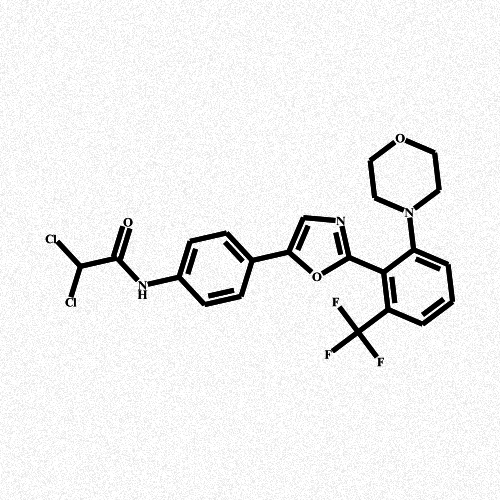
\includegraphics [scale=0.45] {my_folder/images/nh_vert}
	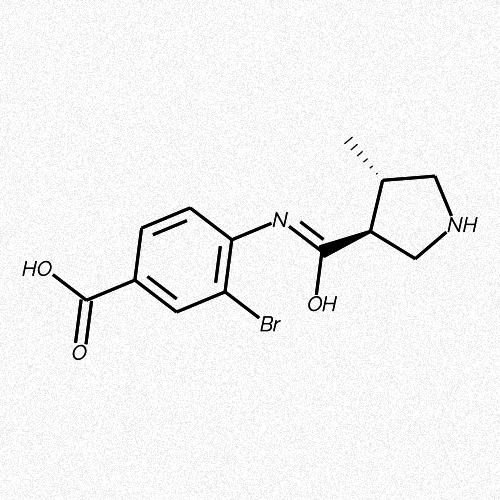
\includegraphics [scale=0.45] {my_folder/images/nh_hor}
	\caption{Изображения молекул, на которых метка атома азота с присоединённым атомом водорода изображена: (1) вертикально, (2) горизонтально} 
	\label{fig:nh}  
\end{figure}

\begin{figure}[h!] 
	\center
	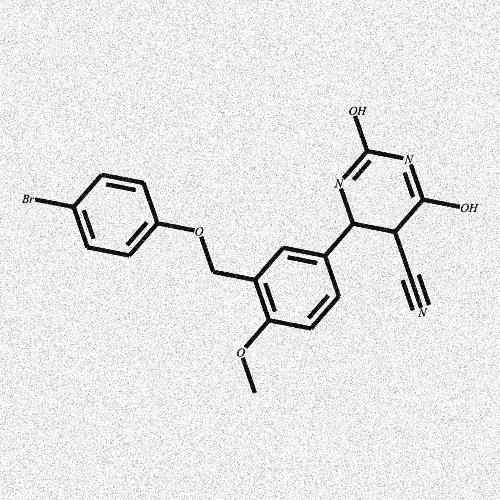
\includegraphics [scale=0.45] {my_folder/images/23bonds}
	\caption{Молекула с двойными и тройными связями. Двойная связь обозначается двумя параллельными отрезками, тройная -- тремя} 
	\label{fig:23bond} 
\end{figure}

Таким образом, программная поддержка алгоритмических решений является крайне трудоёмким процессом, поскольку при появлении новых, пусть даже слабо отличающихся от предыдущих, стандартов рендеринга изображений, в программу-распознаватель придётся дописывать блоки кода, поддерживающие эти изменения.

В то же время решение, построенное с помощью методов машинного обучения, даже не видя каких-то характерных особенностей изображений при обучении, зачастую сможет провести коррректное распознавание. Если же окажется, что изменение слишком сильное, достаточно добавить некоторое количество изображений с новой особенностью в обучающую выборку и дообучить сеть, что требует весьма небольших затрат ресурсов.

Задача распознавания структуры химической молекулы является частью комплексного решения по распознаванию документа и необходима преимущественно для распознавания научных статей по химии, биологии и медицине. Распознавание документов необходимо для следующих целей:
\begin{itemize}
	\item Хранение <<идеальных>> рендеров: пользователь получает возможность читать документы без дефектов. Изображения молекул и другие векторные по своей природе схемы, отпечатанные на бумаге в растровом виде, сохраняются в векторном формате, что позволяет пользователю масштабировать изображение до необходимых ему пределов.
	
	\item Хранение документов в plain-text формате позволяет осуществлять эффективный поиск информации. В частности, модуль распознавания структуры молекулы позволяет искать научные статьи, содержащие информацию о конкретной молекуле. Данная функциональность помогает фармацевтическим исследователям находить интересующие их свойства конкретных веществ, что значительно ускоряет процесс создания лекарственных средств.
\end{itemize}

В рамках данной работы предполагается, что распознавание структуры химической молекулы может производиться как для сканов печатных документов, так и для электронных документов, не содержащих информацию о структуре молекулы в плоском виде.

Таким образом, \textbf{исследование является актуальным}, поскольку построение решения, которое позволяет распознавать структуру химической молекулы на разнообразных данных, поможет создать высококачественный распознаватель документов химической тематики, что в свою очередь значительно улучшит качество и производительность работы исследователей в сфере химии, биологии и фармацевтики.

\textbf{Целью проводимого исследования} является создание описанного ранее решения, замеры его качества, оценка производительности. Также в рамках исследования будет оценена скорость обучения выбранных моделей и \textit{масштабируемость} решения, то есть трудозатраты, требуемые для поддержки дополнительных элементов молекул, таких как RS-стереометки атомов и обозначения смесей различных геометрических изомеров.

\begin{figure}[h!] 
	\center
	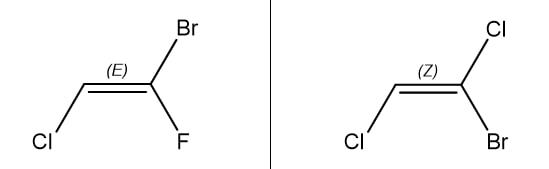
\includegraphics [scale=0.74] {my_folder/images/ez}
	\caption{Изображение молекул с \textit{(E)}, \textit{(Z)} метками \cite{stereochem}}
	\label{fig:ez}  
\end{figure}

\begin{figure}[h!] 
	\center
	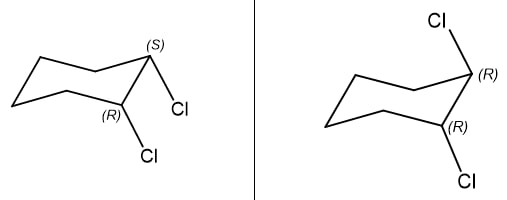
\includegraphics [scale=0.68] {my_folder/images/rs}
	\caption{Изображение молекул с \textit{(R)}, \textit{(S)} метками \cite{stereochem}} 
	\label{fig:rs}  
\end{figure}


% Целью первой главы, как правило, является всесторонний анализ предмета и объекта исследования, второй --- разработка предложений (алгоритмов, технологий и т.п.) по улучшению какого-либо процесса, протекающих с участием предмета и объекта исследования, третьей --- практическая реализация (имплементация) --- предложений (алгоритмов, технологий и т.п.) в виде программного (или иного) продукта, четвертой --- апробация разработанных в работе предложений и выводы целесообразности их дальнейшей разработки (использованию). 


%% Вспомогательные команды - Additional commands
%\newpage % принудительное начало с новой страницы, использовать только в конце раздела
%\clearpage % осуществляется пакетом <<placeins>> в пределах секций
%\newpage\leavevmode\thispagestyle{empty}\newpage % 100 % начало новой строки	    	 % Введение

%% Начало основной части
\chapter{Постановка задачи распознавания молекулы. Методы решения} \label{ch1}

В данной главе приводится постановка задачи распознавания молекулы. Даются определения основных понятий предметной области и описываются существующие решения.

В параграфе \ref{ch1:sec1} приводится постановка задачи распознавания молекулы. Производится описание входных и выходных данных. В параграфе \ref{ch1:sec2} описана общая структура программ, построенных с использованием алгоритмов распознавания геометрических примитивов. Такие программы мы будем называть \textbf{rule-based решениями}. В параграфе \ref{ch1:sec3} описаны различные подходы решения задачии распознавания молекулы с использованием методов машинного обучения -- \textbf{ML-based системы}. В параграфе \ref{ch1:sec4} описано решение на базе нейросети с архитектурой <<трансформер>>. В параграфе \ref{ch1:sec5} приведён алгоритм сборки молекулы из распознанных тех или иным способом примитивов.

\section{Постановка задачи распознавания молекулы} \label{ch1:sec1}
\subsection{Описание входных данных}
На вход задачи подаётся изображение химической молекулы. В рамках данной задачи конкретизируются следующие требования к изображениям:
\begin{itemize}
	\item Молекула является органической. Это означает, что в молекуле присутствуют только атомы, характерные для органических соединений: углерод (C), кислород (O), азот (N), водород (H), фосфор (P), фтор (F), кремний (Si), а также хлор (Cl) и бром (Br).
	\item Молекула может быть стереоизомером: на изображении допускаются сплошные и штрихованные клиновидные связи.
	\item На изображении отрендерена молекула, являющаяся конкретным изомером, то есть не поддерживаются смеси вида \textit{(R), (S), RS, (RS)}. Также не поддерживаются перечёркнутые связи, обозначающие смесь геометрических (E и Z) изомеров.
\end{itemize}

Изображения могут быть получены как из электронных источников литературы, так и из печатных. Допускается наличие дефектов, связанных с небрежным хранением бумажного документа, его возрастом, а также гауссовское зашумление, получаемое в результате процесса сканирования.

Не допускается наличие искажений изображения, получаемых:

\begin{itemize}
	\item при фотографировании на длинной выдержке
	\item при неполном прилегании документа к стеклу сканера.
\end{itemize}

\subsection{Описание выходных данных}
Выходные данные представляют из себя стандартизованный текстовый идентификатор InChI \cite{inchi_trust, inchi_wiki}. Данный идентификатор разработан организациями IUPAC и NIST в течение 2000 -- 2005 годов для обеспечения стандартного и читаемого способа кодирования информации о структуре молекулы и с целью облегчить поиск этой информации в различных базах данных. Он позволяет хранить информацию о структурной формуле, стереоизомерии и наличии изотопов.

Важно отметить, что, тем не менее, InChI не всегда способен однозначно закодировать скелетную формулу. Так, при рисовании алленов зачастую вместо одной из двух клиновидных связей рисуют простую одинарную связь, подразумевая при этом клиновидную. Химики так делают, поскольку знают, что молекула со скелетом такого вида может иметь только одну конкретную геометрическую структуру, в связи с чем достаточно нарисовать только один клин. При этом InChI-представления у этих двух скелетных формул будут разными, хотя молекулы являются одинаковыми. Это явление значительно снижает качество распознавания молекул и будет более подробно показано в подразделе \ref{ch3:sec1}.

\section{Rule-based решения} \label{ch1:sec2}
Для подготовки обзора rule-based решений была использована статья \cite{rajan2020review}. В ней описаны 14 различных программных продуктов, реализованных в рамках rule-based подхода. Каждый продукт имеет свои особенности, которые позволяют ему справляться лучше с теми или иными специфическими свойствами изображения, однако основной конвейер у них общий и состоит из следующих этапов:
\begin{enumerate}[1.]
	\item \textbf{Предобработка}. Данный этап предполагает бинаризацию изображения, то есть его перевод в оттенки серого, сглаживание изображения --  использование антиалиасинга, фильтров Гаусса и т. п., и утончение линий.
    \item \textbf{Поиск стандартных и клиновидных связей}. Данная операция предполагает обнаружение и классификацию связей. Стандартные связи являются совокупностью от одного до трёх параллельных отрезков, поэтому они могут быть обнаружены с применением детектора Хаффа. Штрихованные клиновидные связи могут быть обнаружены как последовательность увеличивающихся в толщине и ориентированных одинаковым образом равнобедренных трапеций. Сплошные клиновидные связи изображаются как равнобедренный треугольник, основание которого много меньше, чем две его остальные стороны.
    \item \textbf{Поиск ароматических соединений}. Ароматические соединения -- это циклические углеводороды, обладающие определёнными химическим свойствами, такими как склонность к реакциям замещения. С точки зрения задачи распознавания важно понимать, что ароматическое соединение представляет может быть изображено в виде формулы Кекуле или формулы Полинга -- таким образом, возникает необходимость поиска окружностей внутри циклов и правильного добавления этих соединений в молекулу.
    
    \begin{figure}[h!] 
    	\center
    	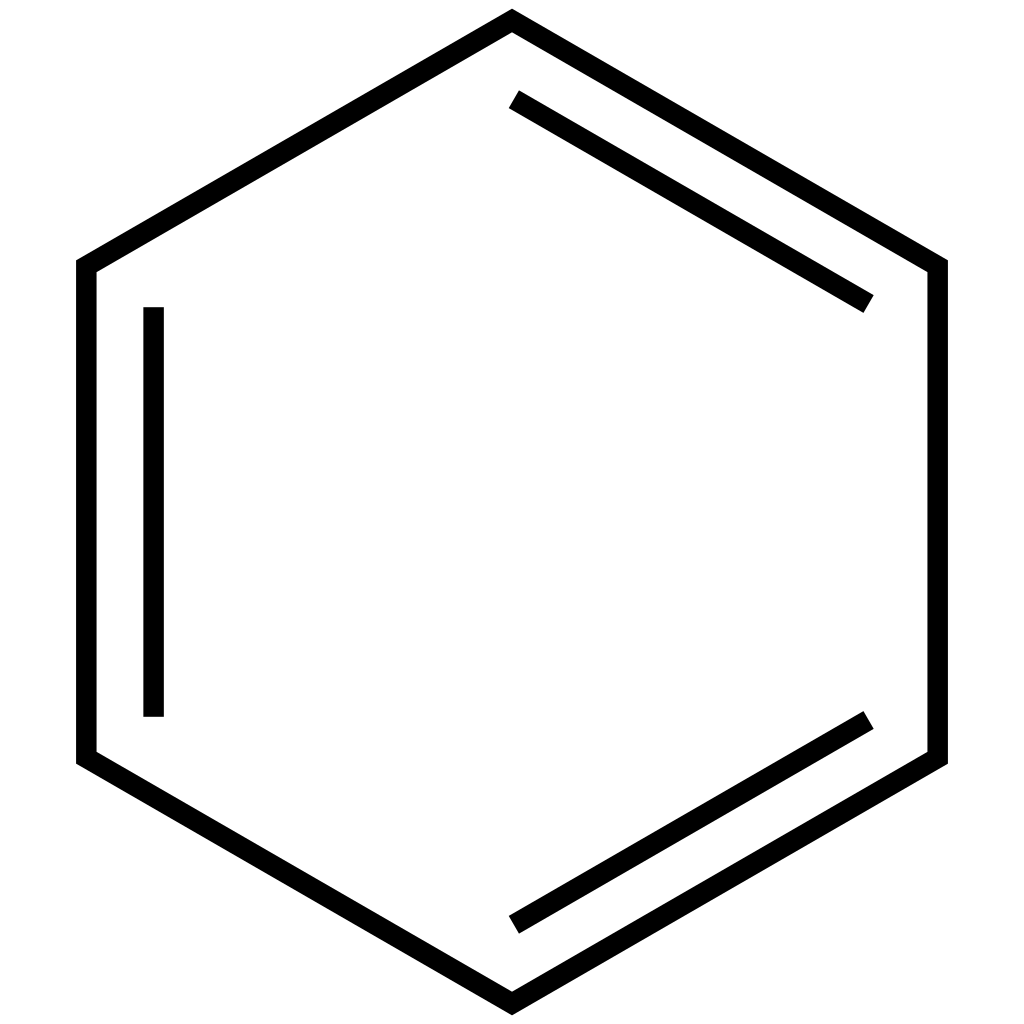
\includegraphics [scale=0.16] {my_folder/images/benzol_kekule}
    	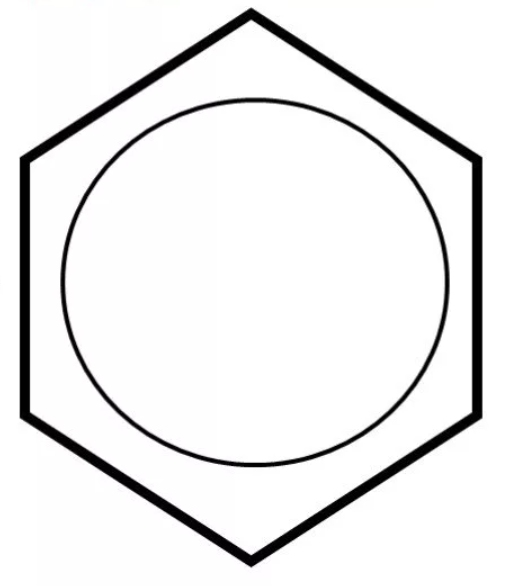
\includegraphics [scale=0.28] {my_folder/images/benzol_poling}
    	\caption{Бензол. (1) Формула Кекуле, (2) Формула Полинга} 
    	\label{fig:benzol}
    \end{figure}
\end{enumerate}

\section{ML-based решения} \label{ch1:sec3}

Согласно \cite{rajan2020review}, до 2019 года было известно два решения, использовавших машинное обучение. Оба продукта представляют из себя совокупность моделей, решающих \textbf{object detection задачу} (см. \ref{ch2:sec1}). Первое из них, OCSR \cite{gkoutos2003chemical}, использовало карты Кохонена для того, чтобы отличать изображения химических молекул от других картинок. Программный продукт ChemOCR использовал машину опорных векторов (\cite{cortes1995support}) для классификации изображений связей.

Первый продукт, полностью построенный на технологиях машинного обучения, называется MSE-DUDL и представлен в 2019 году \cite{staker2019molecular}. Ивзестно, что в основе этого продукта лежит свёрточная сеть на базе U-Net. Модель была натренирована на 57 миллионах изображений, сгенерированных пакетом Indigo.

Второй продукт, Chemgrapher, содержит две сети. Одна отвечает за обнаружение объектов, а вторая -- за их классификацию. Обе сети являются свёрточными, и были натренированы на изображениях, сгенерированных пакетом RDKit. В результате исследований этого решения было выяснено, что сегментирующая нейронная сеть имеет гораздо более низкое качество, чем классифицирующая.

\section{Решение на базе нейросети-трансформера} \label{ch1:sec4}

Стоит отдельно упомянуть решения, построенные на нейросетях с архитектурой <<трансформер>>.

Отличием трансформера от классических CNN и RNN, используемых для решения object detection задачи, является наличие механизма внимания Multi-Head Attention.

Данная архитектура сетей чаще всего применяется при решении задачи машинного перевода. Тем не менее, как и любая нейронная сеть, трансформер может принимать на вход любые конечные последовательности данных, в частности изображения молекул.

Имея в виду основное назначение сетей-трансформеров, будем описывать принцип их работы в терминах задач обработки текста.

\begin{figure}[h!] 
	\center
	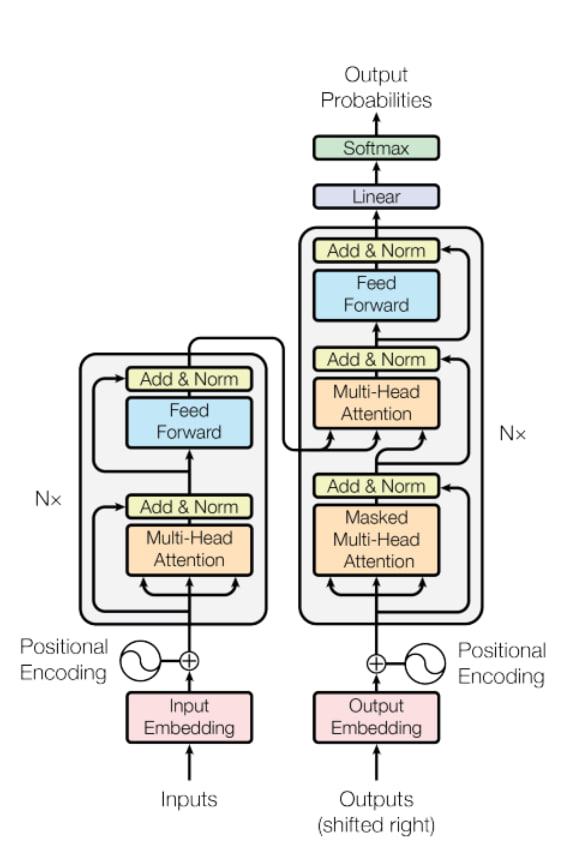
\includegraphics [scale=0.6] {my_folder/images/transformer}
	\caption{Архитектура сети <<трансформер>>} 
	\label{fig:transformer}
\end{figure}

В данной архитектуре все слова параллельно проходят через заданные слои. На пути каждого слова находится слой внимания, суть которого заключается в возможности взаимодействия с другими словами.

На вход слою внимания даются вектора Query и несколько пар Key и Value.  Чаще всего при практическом использовании оказывается, что  Key и Value это один и тот же вектор. Каждый из них преобразуется обучаемым линейным преобразованием, а потом вычисляется скалярное произведение Q со всеми K по очереди, результат этих скалярных произведений подаётся на вход в softmax слой, и с полученными весами все вектора V суммируются в единый вектор. 

\begin{figure}[h!] 
	\center
	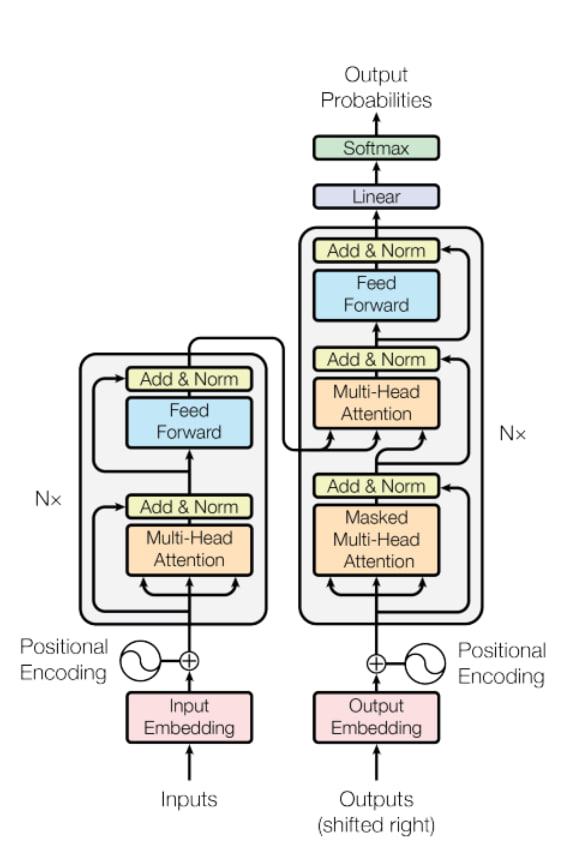
\includegraphics [scale=0.6] {my_folder/images/transformer}
	\caption{Архитектура слоя внимания} 
	\label{fig:attention}
\end{figure}

Данный подход позволяет обучать сеть искать похожие в каком-то смысле слова и таким образом <<уделять внимание>> наиболее значимым словами при произведении машинного перевода. 

Несмотря на то, что трансформеры изначально задумывались как нейросети для машинного перевода, они нашли также применение в других задачах. Например, можно обучить трансформер таким образом, чтобы он на вход получал изображение, а на выход отдавал текстовую последовательность.
Одним из примеров таких сетей является сеть DETR от FacebookResearch \cite{detr}.

На базе трансформера в рамках kaggle-соревнования BMS \cite{bms} было разработано решение, которое конвертирует изображение молекулы \textit{целиком} в InChI-последовательность. Оказалось, что трансформер решает задачу распознавания структуры молекулы даже лучше, чем object detection модель, из чего можно сделать вывод, что механизм внимания позволяет сети обучаться искать взаимосвязь между скелетной формулой и InChI-цепочками. Данное наблюдение ещё раз показвыает способность трансформеров к обучению языкам, поскольку InChI-последовательность, как и скелетная формула, является языком описания структуры молекулы.


\section{Алгоритм сборки молекулы} \label{ch1:sec5}
При решении задачи распознавания молекулы любым из описанных выше способов возникает необходимость собрать молекулу из отдельных примитивов. Приведём здесь алгоритм, который позволяет это делать.

На вход алгоритма подаётся набор изображений связей и меток атомов. Будем строить \textit{граф молекулы} -- граф, в вершинах которого находятся атомы (непомеченные атомы углерода либо другие атомы с указанием названия), а рёбрами которого являются связи.

Такой граф можно передать в один из химических пакетов. В рамках данной работы используется Python-реализация пакета RDKit. Данный пакет позволяет:
\begin{itemize}
	\item строить граф молекулы из таких распространённых форматов, как SMILES, SDF, InChI
	\item добавлять атомы и связи в существующий граф молекулы, а также указывать категорию связи
	\item генерировать текстовые идентификаторы SMILES, SDF, InChI из графа молекулы.
\end{itemize}

Таким образом, для генерации InChI-идентификатора достаточно правильным образом сформировать граф молекулы.

Будем считать, что связи представлены в виде баундбоксов, для которых указана категория связи и её направление. В случае плоской связи достаточно указать направление диагонали, в случае стереосвязи -- её начало и конец. Метки атомов также ожидаются в виде баундобксов, для которых указан текст метки.

Граф строится в несколько этапов.

Первый этап -- построение списка смежности молекулы. Для этого производится двойное вложенное итерирование по списку связей и, если у связей находится общая точка (пересечение баундбоксов с учётом направления связи внутри баундбокса), то точка соединения объявляется новым атомом. Если атом уже существует в списке смежности, то текущая связь добавляется в него. Иначе, создаётся новый элемент в списке смежности и к нему присоединяется две связи.

Второй этап -- поиск висячих вершин, то есть непомеченных атомов, которые связаны только с одним другим атомом.

Третий этап -- сопоставление помеченных и непомеченных атомов. Для этого производится итерирование по всем возможным парам вершин графа молекулы и меток атомов и, если метка расположена достаточно близко к вершине, то считается, что метка относится к данной вершине.

Последний этап -- добавление построенного списка смежности в RDKit-молекулу. После того, как атомы и связи добавлены, необходимо вызвать генератор центров хиральности. Он позволяет сгенерировать данные, необходимые для вывода InChI-идентификатора из информации о клиновидных связях. Важно заметить, что RDKit самостоятельно выводит количество присоединённых атомов водорода из того набора связей, который текущий атом имеет со своими соседями. Это обстоятельство позволяет при классификации меток атомов определять в одну категорию метки с явным указанием присоединённых атомов водорода и без него.

Неприятным моментом является тот факт, что на данном этапе происходят основные потери точности сборки, связанные с неоднозначным соответствием строения химической молекулы и необходимым набором клиновидных связей, о котором упоминалось во введении.

%
%\begin{table} [htbp]% Пример оформления таблицы
%	\centering\small
%	\caption{Представление данных для сквозного примера по ВКР \cite{Peskov2004}}%
%	\label{tab:ToyCompare}		
%		\begin{tabular}{|l|l|l|l|l|l|}
%			\hline
%			$G$&$m_1$&$m_2$&$m_3$&$m_4$&$K$\\
%			\hline
%			$g_1$&0&1&1&0&1\\ \hline
%			$g_2$&1&2&0&1&1\\ \hline
%			$g_3$&0&1&0&1&1\\ \hline
%			$g_4$&1&2&1&0&2\\ \hline
%			$g_5$&1&1&0&1&2\\ \hline
%			$g_6$&1&1&1&2&2\\ \hline		
%		\end{tabular}	
%	\normalsize% возвращаем шрифт к нормальному
%\end{table}


% \firef{} от figure reference
% \taref{} от table reference
% \eqref{} от equation reference


%Формулы могут быть размещены в несколько строк. Чтобы выставить номер формулы напротив средней строки, используйте окружение \verb|multlined| из пакета \verb|mathtools| следующим образом \cite{Ganter1999}:
%
%\begin{equation} 
%\label{eq:fConcept-order-ch1}
%\begin{multlined}
%(A_1,B_1)\leq (A_2,B_2)\; \Leftrightarrow \\  \Leftrightarrow\; A_1\subseteq A_2\; \Leftrightarrow \\ \Leftrightarrow\; B_2\subseteq B_1. 
%\end{multlined}
%\end{equation}


%Используя команду \verb|\labelcref| из пакета \verb|cleveref|, допустимо следующим образом оформлять ссылку на несколько формул:
%(\labelcref{eq:Pi-ch1,eq:fConcept-order-ch1}).
%
%
%\input{my_folder/tex/fig-spbpu-whitehall-three-in-one} % пример подключения 3х иллюстрации в одном рисунке

%Пример ссылок \cite{Article,Book,Booklet,Conference,Inbook,Incollection,Manual,Mastersthesis,Misc,Phdthesis,Proceedings,Techreport,Unpublished,badiou:briefings}, а также ссылок с указанием страниц, на котором отображены номера страниц  \cite[с.~96]{Naidenova2017} или в виде мультицитаты на несколько источников \cites[с.~96]{Naidenova2017}[с.~46]{Ganter1999}. Часть библиографических записей носит иллюстративный характер и не имеет отношения к реальной литературе. 



%\FloatBarrier % заставить рисунки и другие подвижные (float) элементы остановиться

%% Вспомогательные команды - Additional commands
%
%\newpage % принудительное начало с новой страницы, использовать только в конце раздела
%\clearpage % осуществляется пакетом <<placeins>> в пределах секций
%\newpage\leavevmode\thispagestyle{empty}\newpage % 100 % начало новой страницы	         	 % Глава 1
\ContinueChapterBegin % размещать главы <<подряд>> 
\chapter{Построение конвейера машинного обучения. Генерация данных} \label{ch2}

Данная глава посвящена исследованиям, проведённым для построения конвейера машинного обучения. В параграфе \ref{ch2:sec1} приведено описание object detection задачи машинного обучения и выбранной для этого модели. В параграфе \ref{ch2:sec2} описан первоначальный конвейер моделей, с помощью которого предполагалось решать задачу. Описан процесс генерации данных для используемой object detection модели, результаты обучения модели. В параграфе \ref{ch2:sec3} предложены исправления, необходимые для повышения качества обучения модели и  показаны результаты обучения object detection модели на итоговом варианте. Далее, приводится методика генерации данных для обучения вспомогательных сетей, решение об использовании которых было принято по результатам проведённых ранее экспериментов. Показаны результаты обучения вспомогательных моделей.

\section{Object detection задача. Модель Detectron2 Faster R-CNN} \label{ch2:sec1}

Object detection задача состоит в необходимости найти область интереса -- region of interest, ROI в виде баундбокса, то есть прямоугольника, стороны которого параллельны сторонам экрана, и который содержит объект интереса.

Для выполнения данной работы была использована модель Detectron2 Faster R-CNN ResNet 50 FPN \cite{detectron}.

\subsection{Архитектура Detectron2 Faster R-CNN ResNet 50 FPN}

Для того, чтобы детально описать архитектуру сети Detectron2 Faster R-CNN, необходимо сначала описать архитектуру сетей предыдущего поколения R-CNN и Fast R-CNN.

\subsubsection{Архитектура R-CNN}

\textbf{R-CNN}, основоположник модели Faster R-CNN -- одна из первых моделей, применённых для обнаружения объекта на картинке \cite{rcnn}.

Его архитектура состоит из следующих шагов:

\begin{enumerate}[1.]
	\item Определение набора гипотез.
	\item Извлечение из предполагаемых регионов признаков с помощью сверточной нейронной сети и их кодирование в вектор.
	\item Классификация объекта внутри гипотезы на основе вектора из шага 2.
	\item Улучшение (корректировка) координат гипотезы.
	\item Повтор шагов 2-4, пока не будут обработаны все гипотезы.
\end{enumerate}

Опишем каждый этап подробнее.

\begin{itemize}
	\item \textbf{Поиск гипотез}. Изображение на входе первым делом разбивается на маленькие гипотезы разных размеров. Для этого используется алгоритм Selective Search \cite{ssearch}. Таким образом выделяется примерно 2000 разных регионов, которые частично друг друга перекрывают. Для более точной последующей обработки каждая гипотеза дополнительно расширяется на 16 пикселей во всех 4 направлениях -- как бы добавляя \textit{контекст}.
	
	\item \textbf{Кодирование признаков в вектор}. Каждая гипотеза из предыдущего шага независимо и по отдельности друг от друга поступает на вход сверточной нейронной сети. В качестве нее используется архитектура AlexNet без последнего softmax-слоя. Главной задачей сети является кодирование поступаемого изображения в векторное представление, которое извлекается из последнего полносвязного FC7 слоя. Так на выходе получается 4096-размерное векторное представление.
	
	\item \textbf{Классификация}. После получения характеризующего гипотезу вектора становится возможна ее дальнейшая обработка. Для определения, какой именно объект находится в предполагаемом регионе, авторы используют классический метод классификации разделяющими плоскостями на базе SVM. SVM работает по принципу OvR: One vs. Rest -- один против всех, один из методов мультиклассовой классификации. Таким образом, фактически решается задача бинарной классификации -- есть ли конкретный класс объекта внутри предполагаемого региона или нет. Таким образом, выходом является размерный вектор, отображающий уверенность в конкретном классе содержащегося в гипотезе объекта.
	
	\item \textbf{Уточнение гипотез}. 
	Гипотезы, полученные на шаге 1, не всегда содержат правильные координаты, например, объект может быть неудачно <<обрезан>>. Поэтому необходимо их дальнейшее уточнение. Так, гипотезы, содержащие какой-либо объект (наличие объекта определяется на шаге классификации), дополнительно обрабатываются линейной регрессией. То есть гипотезы с классом «фон» не нуждаются в дополнительной обработке регионов, ведь на самом деле там нет объекта.
	
	Каждый объект, специфично для своего класса, имеет определенные размеры и соотношения сторон, поэтому рекомендуется применять собственный регрессор на каждый класс.
	
	В отличие от предыдущего шага, авторы для наилучшей работы используют на входе не вектор из слоя FC7, а карты признаков, извлеченные из последнего MaxPooling слоя (в AlexNet его размерность составляет 256×6×6). Это объясняется тем, что  вектор сохраняет информацию о наличии объекта с какими-то характеристическими подробностями, а карта признаков наилучшим образом сохраняет информацию о местоположении объектов.
	
\end{itemize}

\subsubsection{Архитектура Fast R-CNN}

Данная архитектура является улучшенным вариантом архитектуры R-CNN. Целью её создания было, в первую очередь, ускорение процесса обучения и инференса. Рассмотрим этапы, через которые проходит изображение при обработке Fast R-CNN \cite{fasterrcnn}.

\begin{itemize}
	\item Извлечение карты признаков изображения (не для каждой гипотезы по отдельности, а для всего изображения целиком)
	\item Поиск гипотез -- остался без изменения
	\item Сопоставление каждой гипотезы с местом на карте признаков, то есть использование единого набора выделенных признаков для каждой гипотезы (координаты гипотез можно однозначно сопоставить с местоположением на карте признаков)
	\item Классификация каждой гипотезы и исправление координат ограничивающей рамки (эту часть стало возможным запускать параллельно, поскольку больше нет зависимости от SVM-классификации)
\end{itemize}

В изначальной концепции R-CNN каждая предложенная гипотеза по отдельности обрабатывается с помощью CNN -- этот этап стал бутылочным горлышком для всей архитектуры. Для решения этой проблемы был разработан Region of Interest (RoI) слой. Этот слой позволяет единожды обрабатывать изображение целиком с помощью нейронной сети, получая на выходе карту признаков, которая далее используется для обработки каждой гипотезы.

Основной задачей RoI слоя является сопоставление координат гипотез (координаты баундбоксов) соответствующим координатам карты признаков. Делая <<срез>> карты признаков, RoI слой подает его на вход полносвязному слою для последующего определения класса и поправок к координатам (см. следующие разделы).

В R-CNN использовались отдельные SVM-классификаторы. В Fast R-CNN они заменены одним SoftMax выходом. Отмечается, что при этом потеря точности составляет менее 1\%.

Выход регрессоров обрабатывается с помощью NMS (Non-Maximum Suppression).

\textbf{Multi-task loss}. В одновременном обучении сети для задач регрессии баундбоксов и классификации применяется специальная лосс-функция:

\begin{equation}
	L(p, u, t^u, v) = L_{cls}(P, u) + \lambda_{[u_1]}L_{loc}(t^u, v)
\end{equation},

где:

\begin{itemize}
	\item $\lambda$ -- настройка баланса между функциями потерь регрессора баундбоксов и классификатора
	\item $u$ -- правильный класс
	\item $L_{cls}$ -- функция потерь классификатора: $L_{cls}(P, u) = -\log P_u$
	\item $L_{loc}$ измеряет разницк между целевым значением.
\end{itemize}

$L_{loc}$ является $SmoothL1$-функцией и измеряет разницу между предсказаниями и целевыми значениями:

\begin{equation}
	SmoothL1(x) = 
	\begin{cases}
		\frac{1}{2}x^2, & |x| < 1 \\
		|x| - \frac{1}{2}, & |x| \geq 1
	\end{cases}
\end{equation}


Здесь $x$ обозначает разность целевого значения и предсказания $t_i^u - v_i$.

\subsubsection{Архитектура Faster R-CNN}

Следующим улучшением является изменение алгоритма поиска гипотез. Для этого представим всю систему как композицию двух модулей -- определение гипотез и их обработка. Первый модуль будет реализовываться с помощью \textbf{Region Proposal Network (RPN)}, а второй аналогично Fast R-CNN (начиная с RoI слоя).

Следовательно, в этот раз процесс работы с изображением изменился и теперь происходит таким образом:

\begin{enumerate}[1.]
	\item Извлечение карты признаков изображения c помощью нейронной сети.
	\item Генерация на основе полученной карты признаков гипотез -- определение приблизительных координат и наличие объекта любого класса.
	\item Сопоставление координат гипотез с помощью RoI с картой признаков, полученной на первом шаге.
	\item Классификация гипотез (уже на определение конкретного класса) и дополнительное уточнение координат.
\end{enumerate}

Основное улучшение произошло именно в месте генерации гипотез -- теперь для этого есть отдельная небольшая нейронная сеть, которую назвали Region Proposal Network.

Конечной задачей данного модуля является полноценная замена Selective Search алгоритма. Для более быстрой работы необходимы общие веса с сетью, извлекающей необходимые признаки. Поэтому входом RPN является карта признаков, полученная после этой сети. Авторы оригинальной статьи используют для извлечения признаков сеть VGG16, выходом которой считают последний сверточный слой -- $conv5_3$. Такая сеть имеет следующие характеристики рецептивного поля:

\begin{itemize}
    \item эффективное сжатие (effective strides): 16
    \item размер рецептивного поля (receptive field size): 196.
\end{itemize}

Это значит, что карта признаков будет в 16 раз меньше изначального размера изображения (количество каналов равно 512), а на каждое значение в ее ячейках оказывают влияние пиксели изначального изображения, лежащие в прямоугольнике размером 196×196. Таким образом выходит, что если использовать стандартный вход VGG16 224×224, то на формирование значения центральной ячейки карты признаков (14, 14) будет влиять почти все изображение целиком. На основе полученной карты признаков RPN для каждой ячейки выдает гипотезы (в изначальной реализации) разного размера и соотношения сторон. Так, для стандартного размера это 14×14×9 = 1764 гипотезы!

Полную архитектуру сети Faster R-CNN с описанием слоёв можно найти в Приложении 1 \ref{appendix1}.

\section{Первоначальный конвейер моделей машинного обучения} \label{ch2:sec2}

\subsection{Описание конвейера}
Первоначально планировалось построить конвейер из двух моделей машинного обучения:
\begin{enumerate}[1.]
	\item Faster R-CNN для поиска и классификации связей и поиска меток атомов (без распознавания текста меток). Предполагалось использовать следующий набор категорий:
	\begin{itemize}
		\item Порядок связи: 1-3
		\item Для связи первого порядка -- категория: плоская, клиновидная сплошная или клиновидная штрихованная
		\item Направление связи: одна из диагоналей для стандартной плоской связи, одно из четырёх возможных направлений для клиновидных стереосвязей
		\item Метка атома.
	\end{itemize}
    \item Свёрточная нейронная сеть для классификации текста меток атомов. Поскольку в условиях задачи сказано, что производится распознавание только стереоорганических молекул, количество возможных меток весьма сильно ограничено. Во всём рассматриваемом датасете присутствует 45 различных меток, из них 15 составляют 97\% всего датасета.
\end{enumerate}

\subsection{Подготовка данных}

Для генерации данных используется открытый датасет -- список InChI-идентификаторов из kaggle-соревнования <<BMS>> \cite{bms}.

С помощью пакета RDKit \cite{rdkit} генерируются изображения молекул в формате png размером 500x500 пикселей. Применяются следующие аугментации:

\begin{itemize}
	\item Изменение длины линии связи
	\item Изменение толщины линии связи
	\item Применение разных типов шрифтов, их жирности, курсива и размера
	\item Повороты молекул (при сохранении ориентации меток атомов)
	\item Зашумление изображения гауссовским шумом.
\end{itemize}

При подготовке данных необходимо произвести \textbf{кекулезацию}. Смысл процедуры состоит в том, чтобы заставить RDKit определять категории связей, являющихся частью ароматической системы, как одинарные и двойные, а не ароматические, как это происходит по умолчанию. Категория ароматической связи присваивается по умолчанию, поскольку RDKit, исходя из InChI-представления, определяет набор связей как ароматическое соединение. Название процедуры связано с тем, что молекула, записанная в виде формулы Кекуле, выглядит как обычная молекула с одинарными и двойными связями, а в формуле Полинга всем связям ароматического соединения присваивается одна и та же категория и они в этом смысле неразличимы между собой.

\subsection{Результаты обучения}

\subsubsection{Метрика AP}

Для анализа качества обучения object detection модели используется метрика AP. Данная метрика показывает, насколько точно модель предсказала баундбокс и одновременно с этим угадала категорию объекта интереса.

Метрика вычисляется следующим образом. Если IoU распознанного $i$-го баундбокса больше некототорого значения $x$, строятся графики $precision(confidence \; score)$ и $recall(confidence \; score)$. Из этих двух параметрически заданных графиков получается график $precision(recall)$. Тогда положим:
\begin{equation}
	AP_{i}[@IoU=x] = \int_0^1 \displaystyle precision(recall)drecall
\end{equation}
\begin{equation}
	AP[@IoU=x] = \frac{1}{n} \sum_{i=1}^{n} \displaystyle AP_{i}[@IoU=x]
\end{equation}

\subsubsection{Графики качества и их анализ}

Обучение производилось на 200000 изображениях. Соотношение размеров обучающей и валидационной выборки -- 80/20. Было произведено 140000 итераций. На одну итерацию приходится обработка 1536 ROI. На одном изображении находится в среднем около 50 ROI, что означает, что была произведена 21 эпоха обучения.

В результате обучения был получен следующий график AP50 для валидационной выборки:

\begin{figure}[h!] 
	\center
	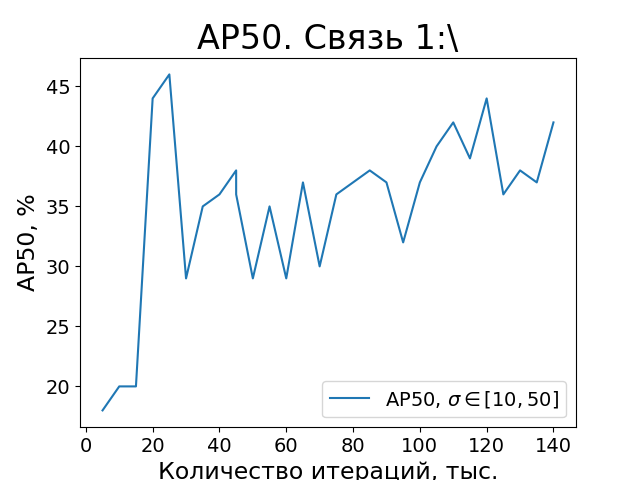
\includegraphics [scale=0.6] {my_folder/images/AP50_first}
	\caption{AP50. Первоначальный вариант обучения Faster R-CNN. Валидационная выборка. Здесь $\sigma$ -- параметр рассеяния гауссовского шума. При генерации датасета изображение зашумливалось в 2 из 3 случаях и, если зашумливалось, то параметр положения $\mu$ гауссовского шума присваивался нулю, а параметр рассеяния $\sigma$ выбирался случайным образом равномерно из диапазона $[10; 50]$}
	\label{fig:AP50_first}
\end{figure}

После того, как был получен такой результат, автор в ручном режиме просмотрел большое количество предсказанных данныхи заметил, что модель практически всегда очень точно определяет границы баундбоксов, но часто путает категории. Отсюда такие низкие показатели метрики AP.

\begin{figure}[h!] 
	\center
	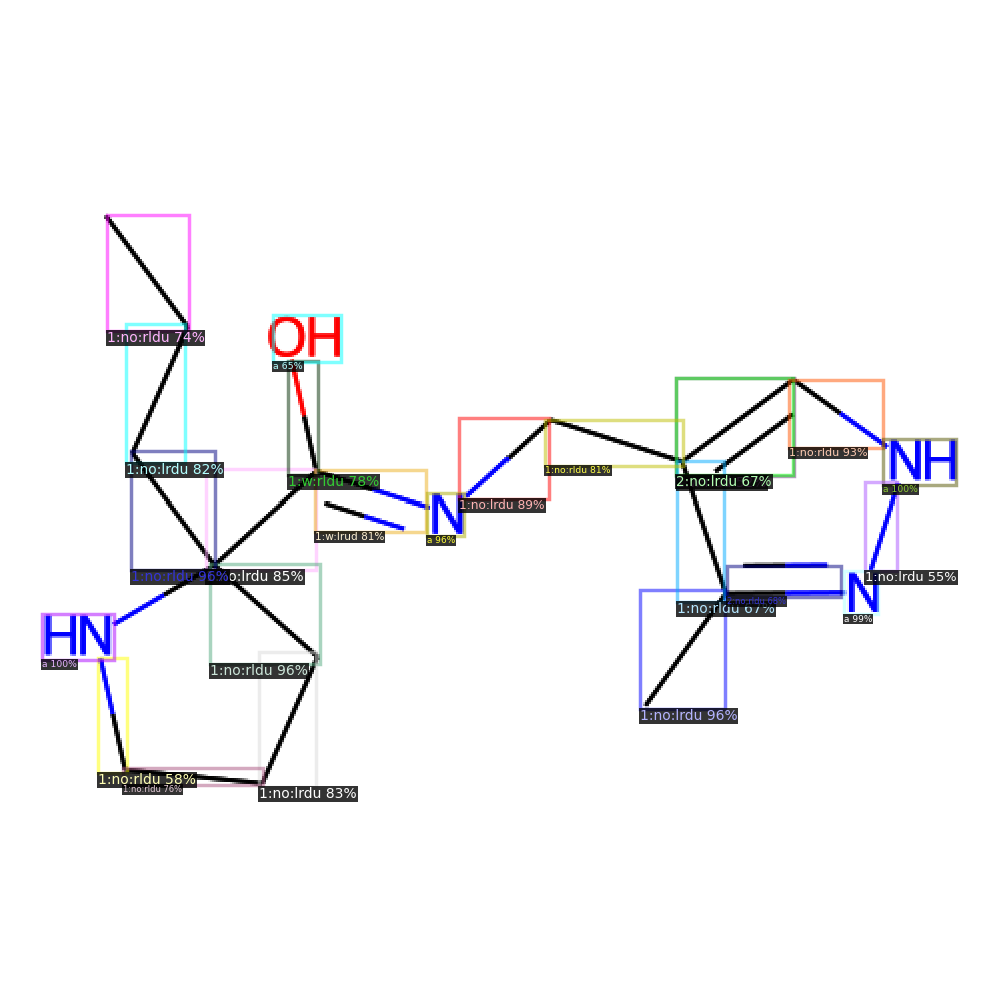
\includegraphics [scale=0.25] {my_folder/images/incorrect_faster_rcnn}
	\caption{Пример результата предсказания. Видно, что двойная связь помечена категорией \textit{1:w:lrud}, что означет сплошную клиновидную связь} 
	\label{fig:rcnn_false}
\end{figure}


\section{Итоговый конвейер моделей машинного обучения} \label{ch2:sec3}
\subsection{Изменения конвейера}
По итогам обучения первоначального варианта было замечено, что модель особенно плохо справляется с определением направления связи внутри баундбокса, в связи с чем было принято решение свести категориальный набор к следующему:

\begin{itemize}
	\item порядок связи: 1-3
	\item метка атома.
\end{itemize}

Ожидается, что уменьшение количества категорий снизит нагрузку на модуль классификации, и тем самым получится повысить качество работы object detection модели.

Для классификации направления связи используется отдельная свёрточная сеть, архитектура которой описана в разделе \ref{ch2:sec3:arch}.


\subsection{Результаты обучения итоговой object detection модели}

Приведём подробные графики всех loss функций.

\begin{figure}[h!] 
	\center
	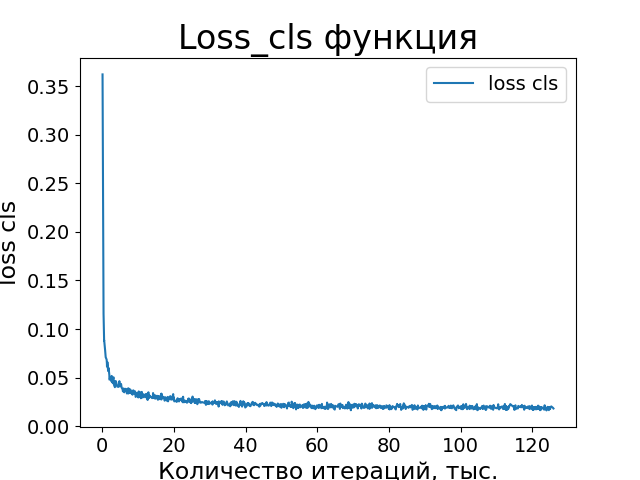
\includegraphics [scale=0.8] {my_folder/images/loss_cls_second}
	\caption{График функции loss\_cls}
	\label{fig:loss_cls}
\end{figure}

\begin{figure}[h!] 
	\center
	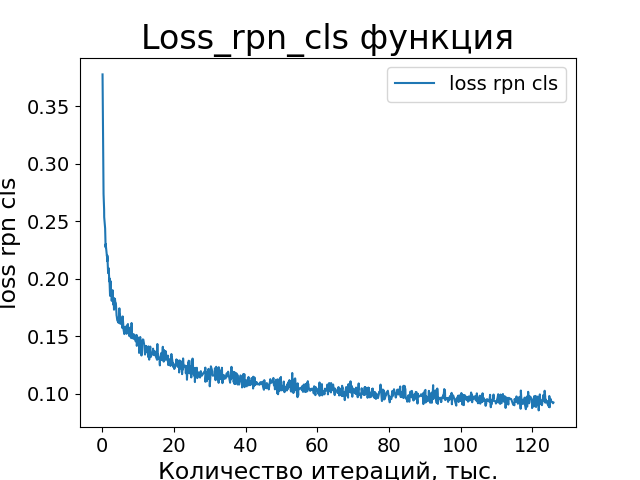
\includegraphics [scale=0.8] {my_folder/images/loss_rpn_cls_second}
	\caption{График функции loss\_rpn\_cls}
	\label{fig:loss_rpn_cls}
\end{figure}

\begin{figure}[h!] 
	\center
	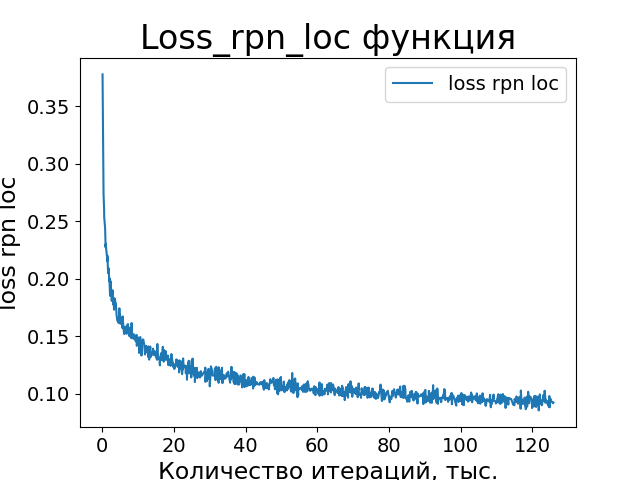
\includegraphics [scale=0.8] {my_folder/images/loss_rpn_loc_second}
	\caption{График функции loss\_rpn\_loc}
	\label{fig:loss_rpn_loc}
\end{figure}

\begin{figure}[h!] 
	\center
	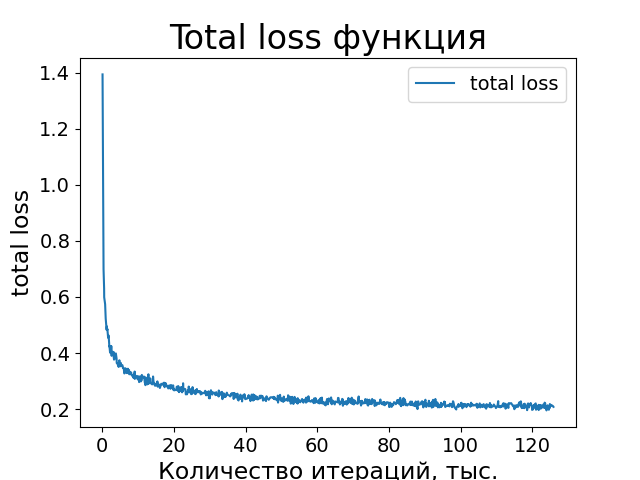
\includegraphics [scale=0.8] {my_folder/images/total_loss_second}
	\caption{График функции total\_loss}
	\label{fig:total_loss}
\end{figure}

Обучение производилось до тех пор, пока все loss-функции не выйдут на асимптоту, поскольку это является критерием окончания обучения модели.

Сопоставим графикам loss-функций графики валидационных метрик AP.

На изображении \ref{fig:AP50_second} приведено два графика AP50 для валидационной выборки. Графики соответствуют разной степени зашумленности изображения. Видно, что, во-первых, качество приблизилось к идеальному: метрика AP50 превосходит 95\% в обоих случаях, а, во-вторых, сеть устойчива к шуму: повышение амплитуды шума в два раза снизило качество обучения не более, чем на 1.5 процентных пункта.

Графики функций потерь приведены для $\sigma \in [10; 200]$.

\begin{figure}[h!] 
	\center
	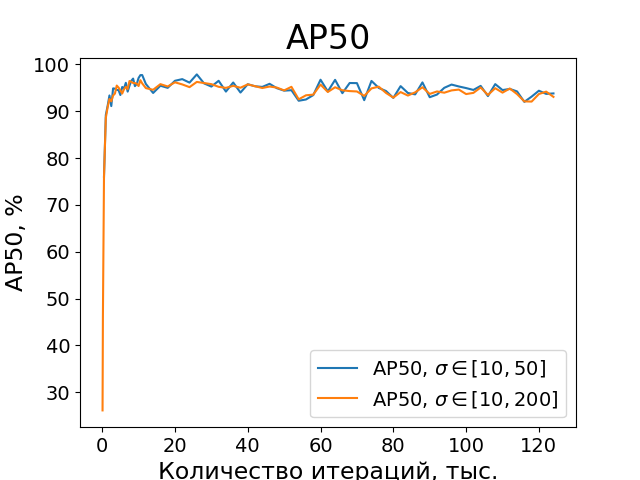
\includegraphics [scale=0.8] {my_folder/images/AP50_second}
	\caption{AP50. Итоговый вариант обучения Faster R-CNN. Валидационная выборка. Приведено два графика для разных степеней зашумленности изображения: $\sigma \in [10; 50], \; \sigma \in [10; 200]$}
	\label{fig:AP50_second}
\end{figure}

Стоит обратить внимание на то, что несмотря на достаточно медленную сходимость сети (выход на асимптоту по всем функциям потерь происходит примерно к 80-100 тысячам итераций), метрики качества выходят на асимптоту гораздо раньше.

\subsection{Архитектура вспомогательных нейронных сетей. Генерация данных} \label{ch2:sec3:arch}

Для классификации направлений связи и меток атомов были обучены две свёрточные нейронные сети с одинаковой архитектурой:
использовались два свёрточных слоя, flatten, dropout и dense слои.

\begin{figure}[h!] 
	\center
	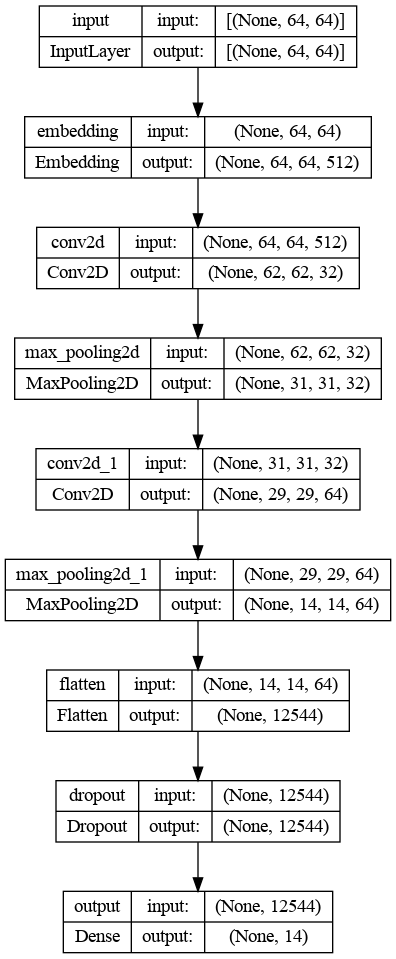
\includegraphics [scale=0.3] {my_folder/images/model_bond}
	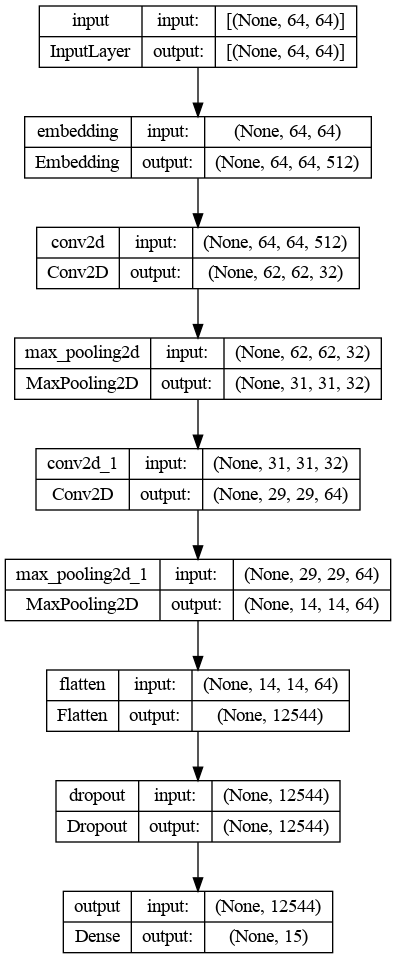
\includegraphics [scale=0.3] {my_folder/images/model_atom}
	\caption{Архитектура CNN для распознавания связей (слева) и меток атомов (справа)}
	\label{fig:AP50_modelbondatom}
\end{figure}

Для генерации обучающих данных использовались ранее сгенерированные для обучения object detection модели изображения. Был сформирован идеально сбалансированный датасет: на каждую категорию сгенерировано по 1000 изображений.

\subsection{Результаты обучения классификаторов}

Обучение производилось в обоих случаях на 50 эпохах, 1500 экземпляров на категорию.

Метрики классификатора категорий связи смотрите в таблице 2.1.

\begin{table}[htbp]% Пример оформления таблицы
	\centering
	\label{tab:bondquality}		
		\begin{tabular}{|c|c|c|}
			\hline
			$F_{1_{\min}}$ & $F_{1_{\max}}$ & $F_{1_{avg}}$ \\
			\hline
			0.97 & 0.99 & 0.98 \\
			\hline
		\end{tabular}
	\caption{Качество обучения классификатора связей}
\end{table}

\begin{figure}[h!] 
	\center
	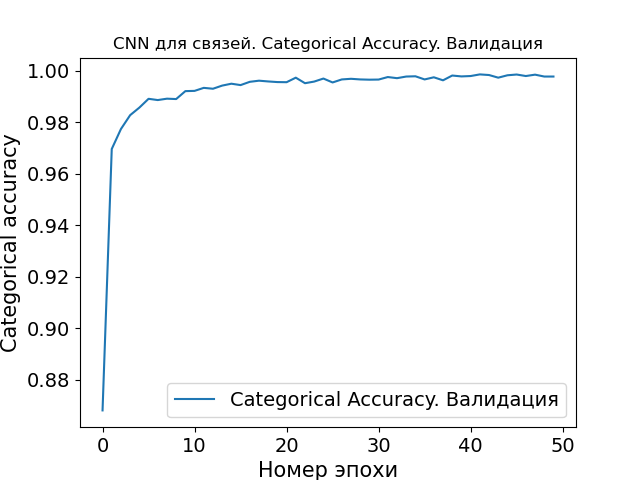
\includegraphics [scale=0.8] {my_folder/images/bonddir_accuracy}
	\caption{График зависимости метрики categorical accuracy от номера эпохи для классификатора категорий связей}
	\label{fig:AP50_bonddir_accuracy}
\end{figure}

\begin{figure}[h!] 
	\center
	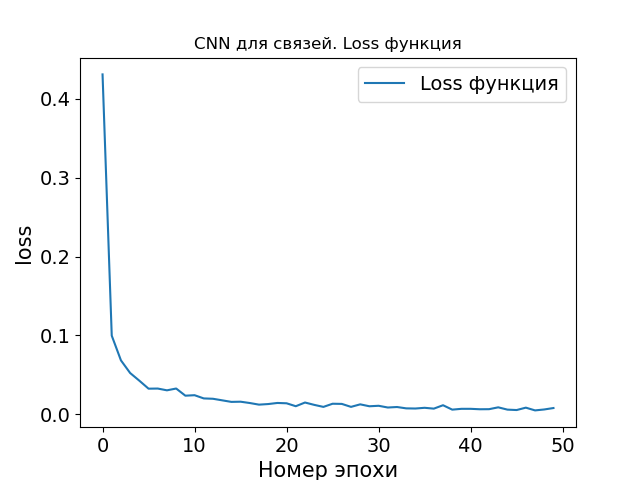
\includegraphics [scale=0.8] {my_folder/images/bonddir_loss}
	\caption{График зависимости функции потерь от номера эпохи для классификатора категорий связей}
	\label{fig:AP50_bonddir_loss}
\end{figure}

Метрики классификатора меток атомов смотрите в таблице 2.2.

\begin{table}[htbp]% Пример оформления таблицы
	\centering
	\label{tab:atomquality}		
	\begin{tabular}{|c|c|c|}
		\hline
		$F_{1_{\min}}$ & $F_{1_{\max}}$ & $F_{1_{avg}}$ \\
		\hline
		0.96 & 0.98 & 0.9\ \\
		\hline
	\end{tabular}
	\caption{Качество обучения классификатора меток атомов}
\end{table}

\begin{figure}[h!] 
	\center
	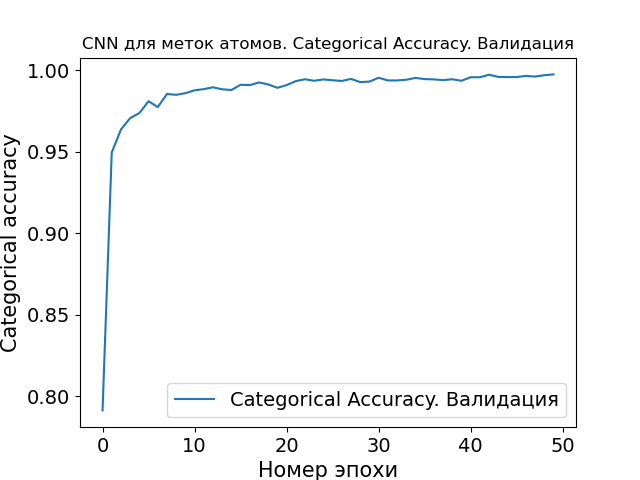
\includegraphics [scale=0.8] {my_folder/images/atom_accuracy}
	\caption{График зависимости метрики categorical accuracy от номера эпохи для классификатора меток атомов}
	\label{fig:AP50_atom_accuracy}
\end{figure}

\begin{figure}[h!] 
	\center
	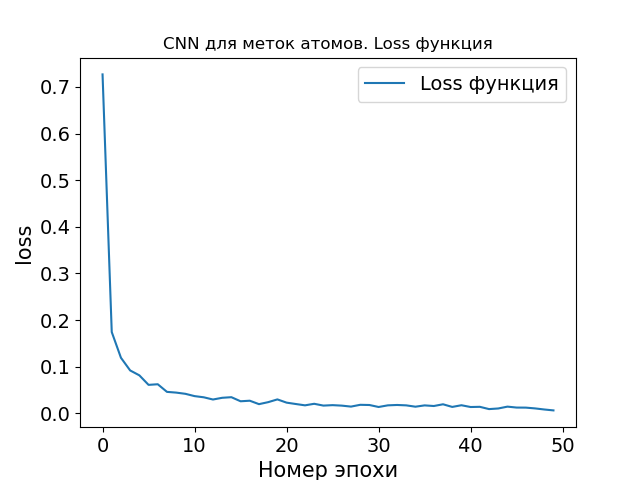
\includegraphics [scale=0.8] {my_folder/images/atom_loss}
	\caption{График зависимости функции потерь от номера эпохи для классификатора меток атомов}
	\label{fig:AP50_atom_loss}
\end{figure}


%\input{my_folder/tex/rules-list-of-environments} % список некоторых окружений
%\input{my_folder/tex/tab-toy-context-minipage} % пример подключения minipage
%\input{my_folder/tex/fig-spbpu-new-bld-autumn-minipage} % пример подключения minipage
%\input{my_folder/tex/rules-theorem-like-expressions} 
%\input{my_folder/tex/theorem-example} %пример оформления теоремы
%\input{my_folder/tex/definition-example} %пример оформления определения
%\input{my_folder/tex/eq-equation-multilined} % пример оформления одиночной формулы в несколько строк
%\input{my_folder/tex/fig-spbpu-sc-four-in-one} % пример подключения 4х иллюстраций в одном рисунке

\FloatBarrier % заставить рисунки и другие подвижные (float) элементы остановиться
\NewPage

	         	 % Глава 2
\chapter{Результаты работы конвейера моделей} \label{ch3}

В данной главе рассматриваются результаты работы конвейера моделей и сборщика графа молекул в совокупности. В параграфе \ref{ch3:sec1} приведено качество работы сборщика молекул. В параграфе \ref{ch3:sec2} приведены следующие метрики: среднее расстояние Левенштейна и процент точных совпадений InChI-идентификаторов. В параграфе \ref{ch3:sec3} показаны характерные примеры, на которых конвейер ошибается, и предложены меры по исправлению некоррректных распознаваний. В параграфе \ref{ch3:sec4} приведены замеры производительности построенного продукта.

\section{Качество сборщика молекул} \label{ch3:sec1}

Сборщик молекул тестировался следующим образом. Из InChI-идентификатора генерировался идеальный вывод конвейера нейросетей. 
Это делалось с помощью функциональности RDKit, позволяющей генерировать векторные изображения молекул. Таким образом, удалось установить точные границы ожидаемых баундбоксов и растеризовать их вместе с самими связями и метками атомов.

Далее полученные данные были переданы на вход сборщика. На выходе был получен InChI-идентификатор, который, в соответствии с ожиданиями, должен точно совпадать со входным идентификатором.

В результате оказалось, что генератор позволяет получить только 92.8\% точных совпадений. При анализе проблемы было выяснено, что 0.8\% несовпадений вызвано некачественной генерацией изображений, когда изображения связей и меток накладываются друг на друга, а остальные 6.4\% вызваны неоднозначностью изображения связи и её метаданных либо неоднозначным соответствием изображения химической молекулы и её физической структурой.

Ярким примером последней ситуации являются изображения алленов. Это соединения, представляющие из себя углеводороды и их замещённые производные с двумя двойными связями у одного атома углерода общей формулы \textbf{RR'C=C=CR''R'''} \cite{allenes}. Известно, что у таких соединений плоскости, в которых находятся атомы \textbf{R, R', C} и \textbf{C, R'', R'''} соответственно, являются ортогональными. Для того, чтобы отразить эту ортогональность на рисунке, необходимо нарисовать две клиновидных связи. Однако из определения алленов понятно, что молекула, состоящая из двух двойных соединяющих атомы углеродов связей, из концов которых выходят ещё по две одинарные связи, обязательно будет являться именно алленом, а не каким-то другим соединением. Поэтому достаточно указывать только один клин -- для того, чтобы определить, какой из атомов -- R или R'  -- находится ближе к наблюдателю, а какой дальше. Таким образом одну и ту же молекулу можно изобразить как минимум тремя способами \footnote{На самом деле таких способов шесть. Можно указывать клиновидность связей, находящихся в правой части изображения -- \textbf{CR''} и \textbf{CR'''}}.

\begin{figure}[ht!] 
	\center
	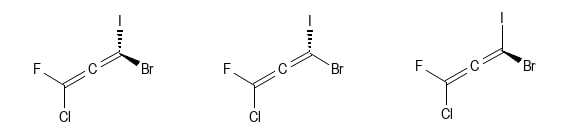
\includegraphics [scale=1.0] {my_folder/images/allene}
	\caption{Три разных изображения одного и того же аллена}
	\label{fig:allenes}
\end{figure}
	
\section{Качество конвейера моделей} \label{ch3:sec2}
Для проведения качественного тестирования моделей были использованы данные, ранее не задействованные при обучении. Было взято 20000 разнообразных молекул и посчитано среднее расстояние Левенштейна. Оно составило 4.32 редакционных изменения.

Процент точных совпадений молекул составил 81.8\%. Учитывая, что точность генератора составляет 92.8\%, можно сделать вывод, что истинная точность конвейера моделей составляет около 81.8\%, что является отличным показателем для object detection задачи, поскольку задача распознавания при таком подходе состоит из большого числа распознаваний, в каждом из которых есть шанс ошибиться и, таким образом, предоставить неточное предсказание.

\section{Типовые ошибки конвейера. Методы устранения} \label{ch3:sec3}

Наиболее часто встречающиеся ошибки связаны с распознаванием меток атомов кислорода и азота с указанием атомов водорода -- $O, NH, NH_2$. Причина заключается в том, что обучающая выборка является несбалансированной: количество меток атомов в несколько раз меньше, чем количество меток связей. Для решения данной проблемы необходимо генерировать набор данных, содержащий большее количество меток атомов при том же количестве связей. Реализация данной функциональности предполагает разработку алгоритма, который сможет менять атомы углерода на другие атомы, соблюдая при этом требования, касающие валентности: количество связей, которые исходят из данного атома, должно быть в списке возможных валентностей. Такой алгоритм может быть реализован при дальнейщих исследованиях в рамках данной работы.

\begin{figure}[ht!] 
	\center
	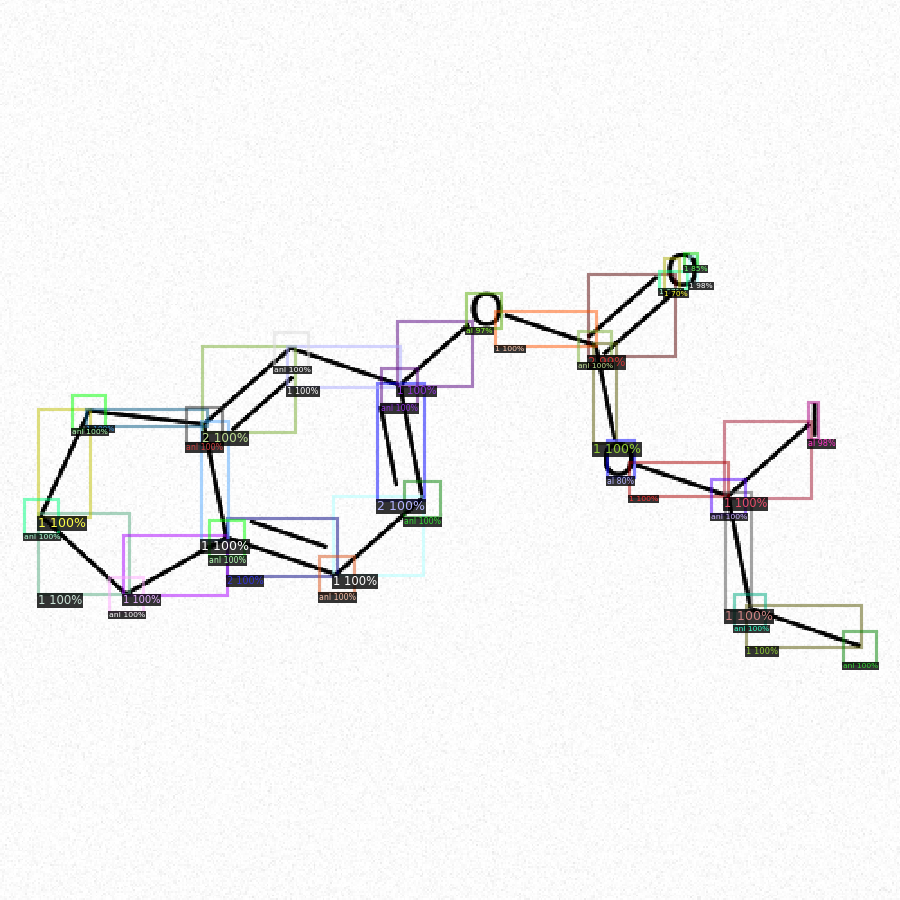
\includegraphics [scale=0.25] {my_folder/images/inference1}
	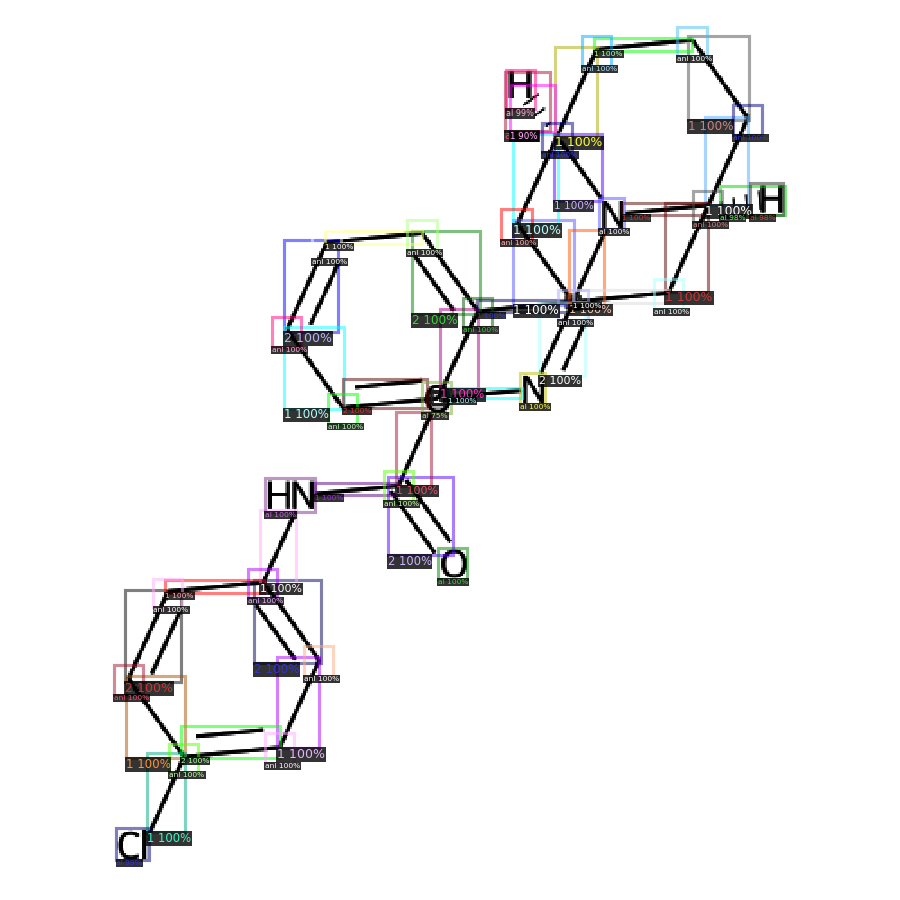
\includegraphics [scale=0.25] {my_folder/images/inference2}
	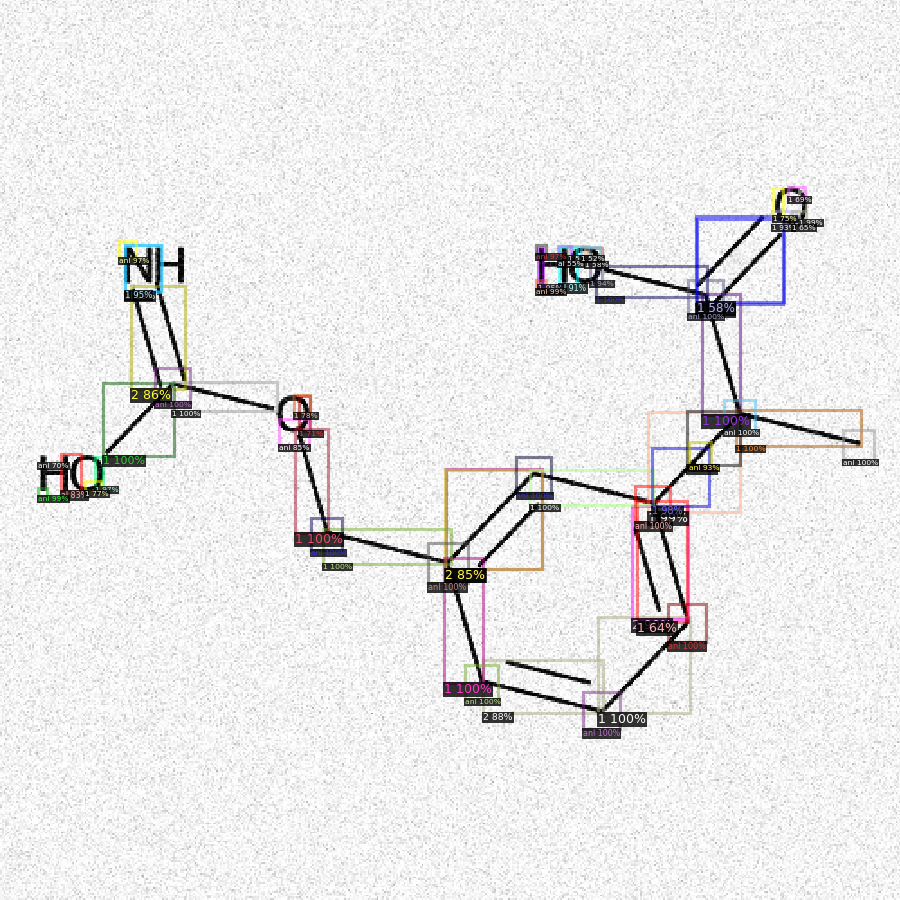
\includegraphics [scale=0.28] {my_folder/images/inference3}
	\caption{Типовые ошибки распознавания Faster R-CNN: некорректно построенные баундбоксы атомов (1) кислорода, (2) водорода, (3) азота}
	\label{fig:mistake}
\end{figure}

Подобные ошибки происходят приблизительно в одном из 15-20 случаев.

\section{Производительность решения} \label{ch3:sec4}

Были произведены замеры производительности на ноутбуке следующей конфигурации:

\begin{itemize}
	\item CPU: AMD Ryzen 5 5600H
	\item GPU: Nvidia GeForce RTX3050
	\item RAM: 16 Gb
\end{itemize}

Для данной конфигурации была производительность решения составила 3.11 изображений в секунду. Из них 45\% уходит на операции RDKit по добавлению элементов во внутреннее представление молекулы и её валидацию. Также около 8\% уходит на обмен данными между CPU и GPU, а оставшиеся 47\% занимает инференс моделей и сборка графа молекулы.


%\FloatBarrier % заставить рисунки и другие подвижные (float) элементы остановиться


%% Вспомогательные команды - Additional commands
%
%\newpage % принудительное начало с новой страницы, использовать только в конце раздела
%\clearpage % осуществляется пакетом <<placeins>> в пределах секций
%\newpage\leavevmode\thispagestyle{empty}\newpage % 100 % начало новой страницы           	 % Глава 3
%\input{my_folder/chapter4}           	 % Глава 3
\ContinueChapterEnd % завершить размещение глав <<подряд>>
%% Завершение основной части

\chapter*{Заключение} \label{ch-conclusion}
\addcontentsline{toc}{chapter}{Заключение}	% в оглавление 

В результате проделанной работы был разработан программный продукт, который позволяет распознавать структуру химической молекулы с применением object detection подхода с точностью 81.8\%. Было проведено исследование, результатом которого стало понимание особенностей работы object detection модели Detectron2 Faster R-CNN на изображениях химических молекул.

Учитывая хорошую разделимость этих данных, можно сделать вывод, что модуль классификации Detectron2 достаточно плохо справляется с возложенной на него обязанностью. Однако регрессор баундбоксов работает очень качественно, в связи с чем можно дать общую рекомендацию по применению таких сетей.

Данная сеть обучается очень быстро и не склонна существенно улучшать качество работы после первых нескольких тысяч итераций, несмотря на то, что loss-функция выходит на асимптоту только приблизительно к статысячной итерации. Стоит обучать такую сеть на поиск баундбоксов, а задачу классификации отдавать в следующую сеть, скорее всего простую по своей структуре. Таким образом, удастся качественно выполнить поставленную задачу и, несмотря на кажущуюся громоздкость и дублирование функциональности двух моделей, практически не потерять в производительности инференса.

Также благодаря такому подходу можно добавить распознавание новых особенностей связей и меток атомов путём минимальных усилий: добавления категорий в классификаторы и сборщик молекул. Обучение классификаторов с нуля даже на CPU занимает не более, чем несколько десятков минут.

Кроме того, в построенном решении найдены проблемные места и даны рекомендации по их устранению и дальнейшим исследованиям: сеть иногда распознаёт очень большое количество баундбоксов на метке атома кислорода и в целом склонна к некорректному распознаванию меток атомов. Это связано с тем, что образцов меток атомов у сети во много раз меньше, чем образцов связей, в связи с чем сеть недоучивается распознавать метки атомов, и вместо них видит связи. Для исправления этой ситуации необходимо реализовать генератор химических соединений, который позволит создавать химически корректные молекулы с большим числом атомов с указываемыми метками -- преимущественно азот, кислород и водород.
        	 % Заключение

%% Наличие следующих перечней не исключает расшифровку сокращения и условного обозначения при первом упоминании в тексте!
%\input{my_folder/acronyms}		         % Необязательная рубрика! Список сокращений и условных обозначений

%\input{my_folder/dictionary}    		 % Необязательная рубрика! Словарь терминов
% По порядку после Списка сокращений и условных обозначений, если есть.	


\input{my_folder/references}		     % Список литературы

% Здесь можно поместить список иллюстративного материала

\appendix % не редактировать / keep unmodified


\chapter{Архитектура Faster R-CNN} \label{appendix1}							% 
%\addcontentsline{toc}{chapter}{Архитектура Faster R-CNN}	% Добавляем его в оглавление

Полная архитектура Faster R-CNN выглядит следующим образом:

\begin{figure}
%	\center
	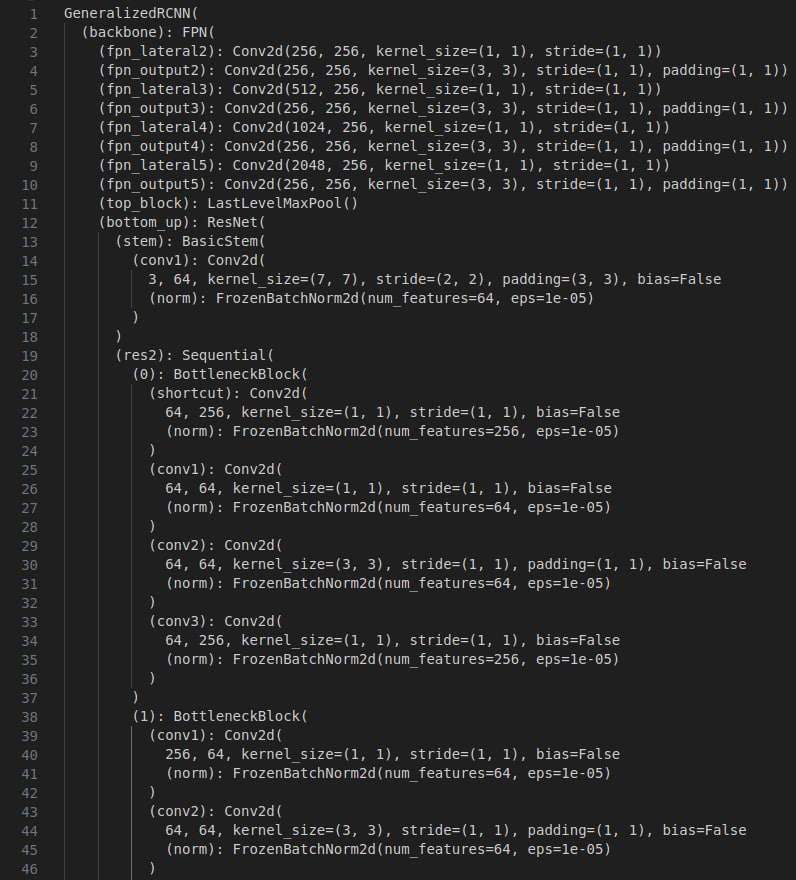
\includegraphics [scale=0.3]{my_folder/images/arch1}
	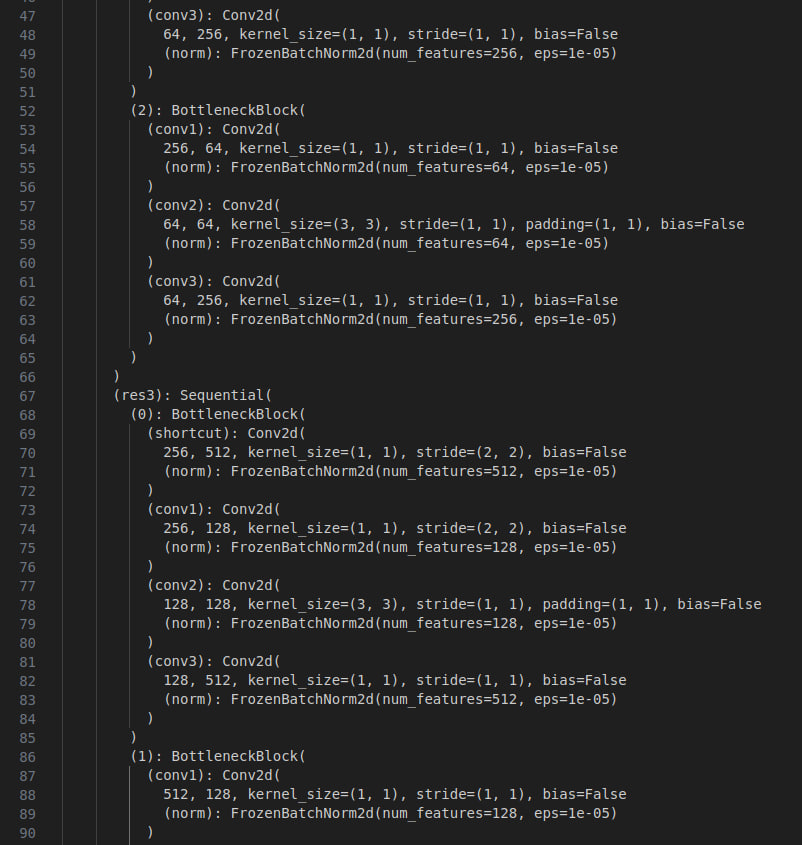
\includegraphics [scale=0.3]{my_folder/images/arch2}
	\label{fig:arch12}
	\caption{Архитектура Faster R-CNN (1)}
\end{figure}
\begin{figure}
%	\center
	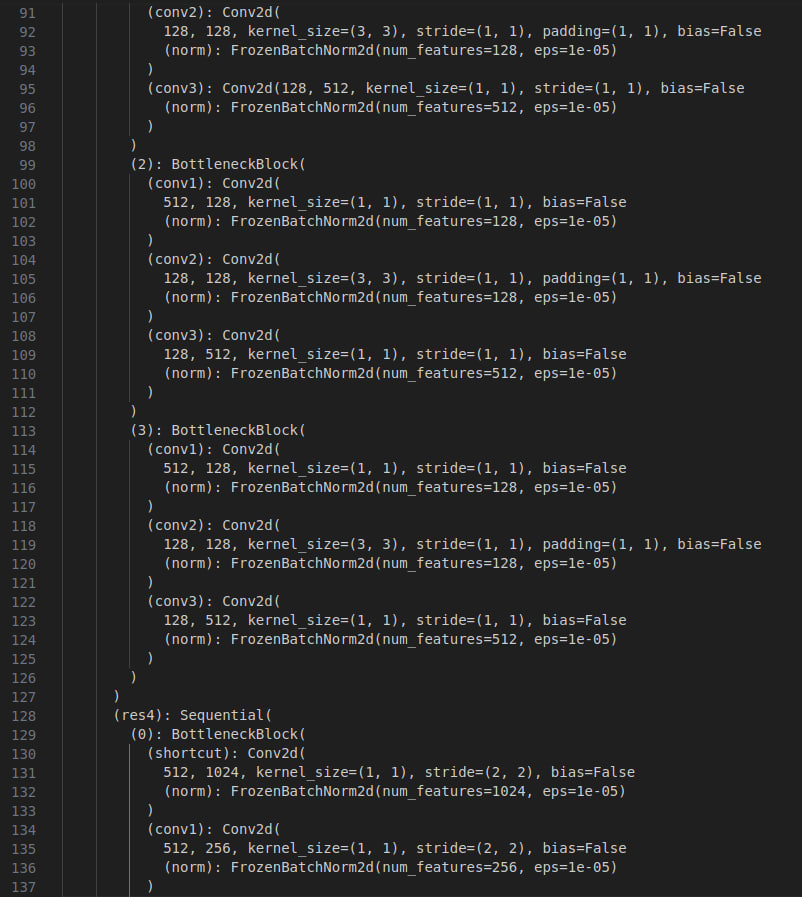
\includegraphics [scale=0.3]{my_folder/images/arch3}
	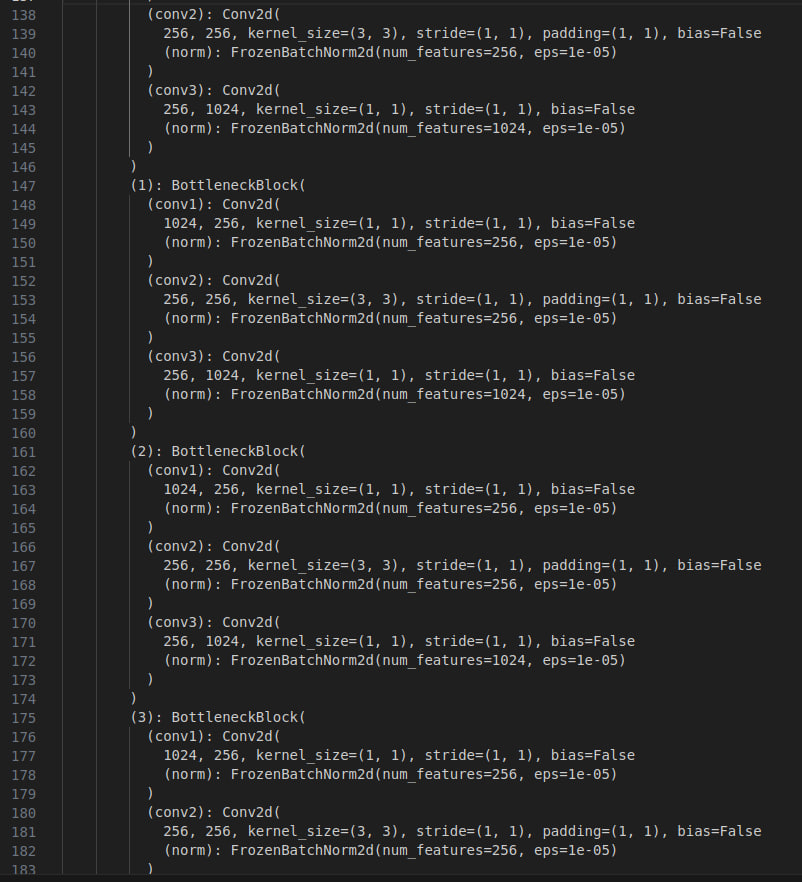
\includegraphics [scale=0.3]{my_folder/images/arch4}
	\label{fig:arch34}
	\caption{Архитектура Faster R-CNN (2)}
\end{figure}
\begin{figure}
%	\center
	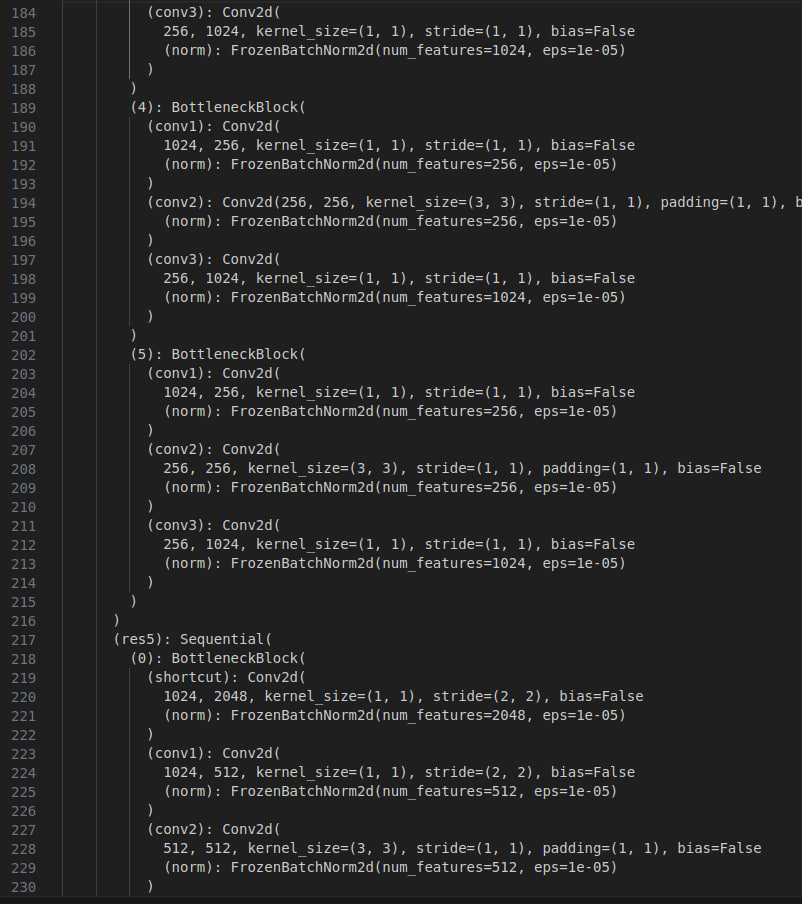
\includegraphics [scale=0.3]{my_folder/images/arch5}
	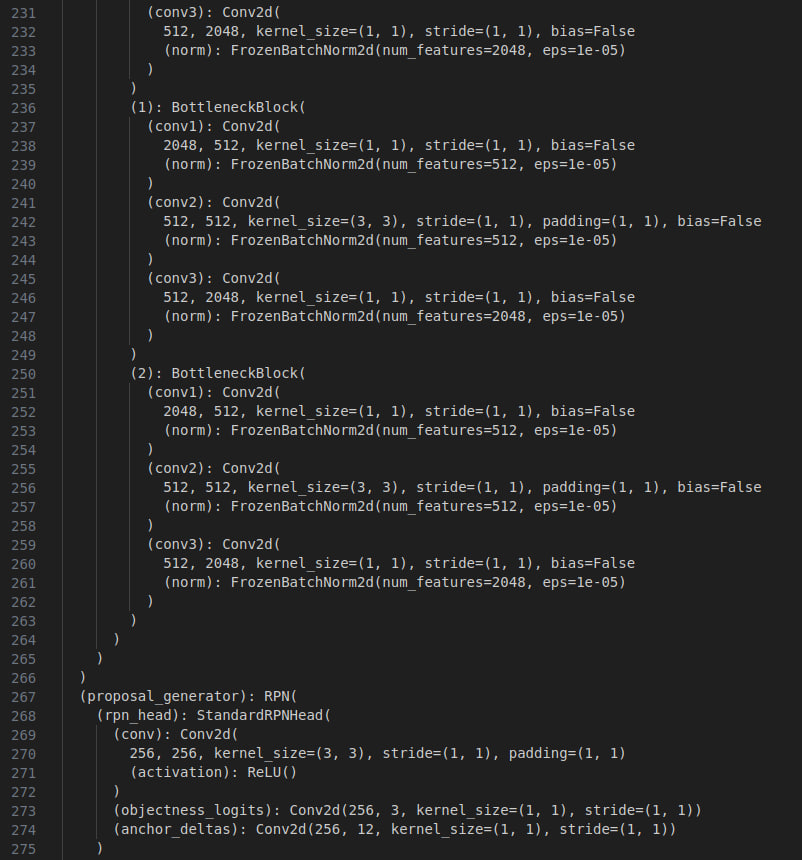
\includegraphics [scale=0.3]{my_folder/images/arch6}
	\label{fig:arch56}
	\caption{Архитектура Faster R-CNN (3)}
\end{figure}
\begin{figure}
%	\center
	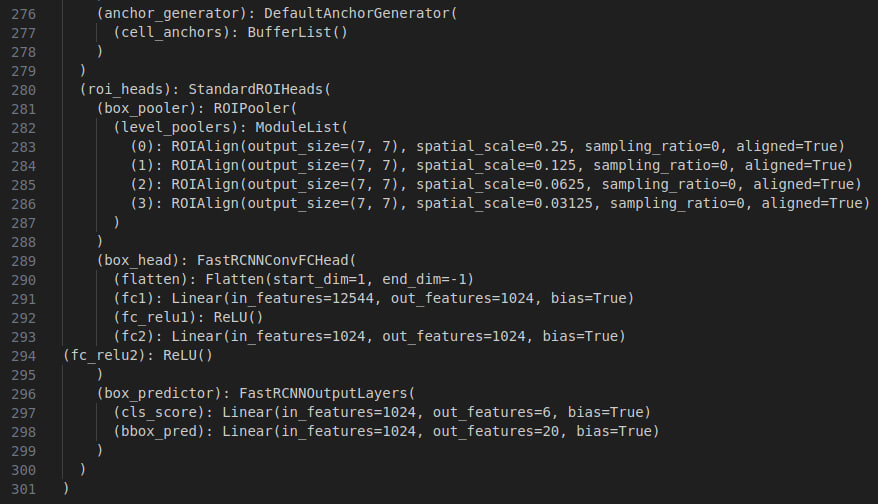
\includegraphics [scale=0.6]{my_folder/images/arch7}
	\caption{Архитектура Faster R-CNN (4)}
	\label{fig:arch7}
\end{figure}
%
%% В случае, когда таблица (рисунок) размещаются на последней странице, для переноса названия приложения на новую строку используем:
%\NewPage % начать новое приложение с новой страницы 			     % Приложение 1
%
%\chapter{Некоторые дополнительные примеры}\label{appendix-extra-examples}							% 


			 	 % Приложение 2


\end{document} % конец документа


%%% Удачной защиты ВКР! - Good luck on the thesis defense!
%%
%%% Поддержать проект
%%
%% Запросы на добавление / изменение просим писать на следующей странице:
%% https://github.com/ParkhomenkoV/SPbPU-student-thesis-template/issues
%%
%% Список пожеланий в файле шаблона <<TO-DO-list.tex>>
%%
%% Благодарности просим указывать в виде 
%%
%% 1. Добавление <<Звезды>> проекту https://github.com/ParkhomenkoV/SPbPU-student-thesis-template/stargazers
%%
%% 2. Добавления <<Сердечка>> и репоста проекта в социальных сетях:
%%		https://vk.com/latex_polytech 
%%		https://www.fb.com/groups/latex.polytech
%%

%%% Support project
%%
%% Requests on adding / modifications is better to be publishen on the following web-page:
%% https://github.com/ParkhomenkoV/SPbPU-student-thesis-template/issues
%%
%% Wishlist is in the template's file called <<TO-DO-list.tex>>
%%
%% Acknowledgements are better to be done in the form of 
%%
%% 1. Adding <<Star>> to the project https://github.com/ParkhomenkoV/SPbPU-student-thesis-template/stargazers
%%
%% 2. Adding <<Likes>> and Project repost in the social networks:
%%		https://vk.com/latex_polytech 
%%		https://www.fb.com/groups/latex.polytech
%% 

% Check list при передаче ВКР:
% - Количество страниц в Задании 2. Если нет, то комментирование последней строки в my_task.tex
% - Зачистка всех вспомогательных файлов (Clear auxilary files) и компиляция ВКР не менее 3х раз